% Options for packages loaded elsewhere
% Options for packages loaded elsewhere
\PassOptionsToPackage{unicode}{hyperref}
\PassOptionsToPackage{hyphens}{url}
%
\documentclass[
  ignorenonframetext,
  aspectratio=169,
]{beamer}
\newif\ifbibliography
\usepackage{pgfpages}
\setbeamertemplate{caption}[numbered]
\setbeamertemplate{caption label separator}{: }
\setbeamercolor{caption name}{fg=normal text.fg}
\beamertemplatenavigationsymbolsempty
% remove section numbering
\setbeamertemplate{part page}{
  \centering
  \begin{beamercolorbox}[sep=16pt,center]{part title}
    \usebeamerfont{part title}\insertpart\par
  \end{beamercolorbox}
}
\setbeamertemplate{section page}{
  \centering
  \begin{beamercolorbox}[sep=12pt,center]{section title}
    \usebeamerfont{section title}\insertsection\par
  \end{beamercolorbox}
}
\setbeamertemplate{subsection page}{
  \centering
  \begin{beamercolorbox}[sep=8pt,center]{subsection title}
    \usebeamerfont{subsection title}\insertsubsection\par
  \end{beamercolorbox}
}
% Prevent slide breaks in the middle of a paragraph
\widowpenalties 1 10000
\raggedbottom
\AtBeginPart{
  \frame{\partpage}
}
\AtBeginSection{
  \ifbibliography
  \else
    \frame{\sectionpage}
  \fi
}
\AtBeginSubsection{
  \frame{\subsectionpage}
}
\usepackage{iftex}
\ifPDFTeX
  \usepackage[T1]{fontenc}
  \usepackage[utf8]{inputenc}
  \usepackage{textcomp} % provide euro and other symbols
\else % if luatex or xetex
  \usepackage{unicode-math} % this also loads fontspec
  \defaultfontfeatures{Scale=MatchLowercase}
  \defaultfontfeatures[\rmfamily]{Ligatures=TeX,Scale=1}
\fi
\usepackage{lmodern}

\ifPDFTeX\else
  % xetex/luatex font selection
\fi
% Use upquote if available, for straight quotes in verbatim environments
\IfFileExists{upquote.sty}{\usepackage{upquote}}{}
\IfFileExists{microtype.sty}{% use microtype if available
  \usepackage[]{microtype}
  \UseMicrotypeSet[protrusion]{basicmath} % disable protrusion for tt fonts
}{}
\makeatletter
\@ifundefined{KOMAClassName}{% if non-KOMA class
  \IfFileExists{parskip.sty}{%
    \usepackage{parskip}
  }{% else
    \setlength{\parindent}{0pt}
    \setlength{\parskip}{6pt plus 2pt minus 1pt}}
}{% if KOMA class
  \KOMAoptions{parskip=half}}
\makeatother


\usepackage{longtable,booktabs,array}
\usepackage{calc} % for calculating minipage widths
\usepackage{caption}
% Make caption package work with longtable
\makeatletter
\def\fnum@table{\tablename~\thetable}
\makeatother
\usepackage{graphicx}
\makeatletter
\newsavebox\pandoc@box
\newcommand*\pandocbounded[1]{% scales image to fit in text height/width
  \sbox\pandoc@box{#1}%
  \Gscale@div\@tempa{\textheight}{\dimexpr\ht\pandoc@box+\dp\pandoc@box\relax}%
  \Gscale@div\@tempb{\linewidth}{\wd\pandoc@box}%
  \ifdim\@tempb\p@<\@tempa\p@\let\@tempa\@tempb\fi% select the smaller of both
  \ifdim\@tempa\p@<\p@\scalebox{\@tempa}{\usebox\pandoc@box}%
  \else\usebox{\pandoc@box}%
  \fi%
}
% Set default figure placement to htbp
\def\fps@figure{htbp}
\makeatother


% definitions for citeproc citations
\NewDocumentCommand\citeproctext{}{}
\NewDocumentCommand\citeproc{mm}{%
  \begingroup\def\citeproctext{#2}\cite{#1}\endgroup}
\makeatletter
 % allow citations to break across lines
 \let\@cite@ofmt\@firstofone
 % avoid brackets around text for \cite:
 \def\@biblabel#1{}
 \def\@cite#1#2{{#1\if@tempswa , #2\fi}}
\makeatother
\newlength{\cslhangindent}
\setlength{\cslhangindent}{1.5em}
\newlength{\csllabelwidth}
\setlength{\csllabelwidth}{3em}
\newenvironment{CSLReferences}[2] % #1 hanging-indent, #2 entry-spacing
 {\begin{list}{}{%
  \setlength{\itemindent}{0pt}
  \setlength{\leftmargin}{0pt}
  \setlength{\parsep}{0pt}
  % turn on hanging indent if param 1 is 1
  \ifodd #1
   \setlength{\leftmargin}{\cslhangindent}
   \setlength{\itemindent}{-1\cslhangindent}
  \fi
  % set entry spacing
  \setlength{\itemsep}{#2\baselineskip}}}
 {\end{list}}
\usepackage{calc}
\newcommand{\CSLBlock}[1]{\hfill\break\parbox[t]{\linewidth}{\strut\ignorespaces#1\strut}}
\newcommand{\CSLLeftMargin}[1]{\parbox[t]{\csllabelwidth}{\strut#1\strut}}
\newcommand{\CSLRightInline}[1]{\parbox[t]{\linewidth - \csllabelwidth}{\strut#1\strut}}
\newcommand{\CSLIndent}[1]{\hspace{\cslhangindent}#1}



\setlength{\emergencystretch}{3em} % prevent overfull lines

\providecommand{\tightlist}{%
  \setlength{\itemsep}{0pt}\setlength{\parskip}{0pt}}



 


\makeatletter
\@ifpackageloaded{caption}{}{\usepackage{caption}}
\AtBeginDocument{%
\ifdefined\contentsname
  \renewcommand*\contentsname{Table of contents}
\else
  \newcommand\contentsname{Table of contents}
\fi
\ifdefined\listfigurename
  \renewcommand*\listfigurename{List of Figures}
\else
  \newcommand\listfigurename{List of Figures}
\fi
\ifdefined\listtablename
  \renewcommand*\listtablename{List of Tables}
\else
  \newcommand\listtablename{List of Tables}
\fi
\ifdefined\figurename
  \renewcommand*\figurename{Figure}
\else
  \newcommand\figurename{Figure}
\fi
\ifdefined\tablename
  \renewcommand*\tablename{Table}
\else
  \newcommand\tablename{Table}
\fi
}
\@ifpackageloaded{float}{}{\usepackage{float}}
\floatstyle{ruled}
\@ifundefined{c@chapter}{\newfloat{codelisting}{h}{lop}}{\newfloat{codelisting}{h}{lop}[chapter]}
\floatname{codelisting}{Listing}
\newcommand*\listoflistings{\listof{codelisting}{List of Listings}}
\makeatother
\makeatletter
\makeatother
\makeatletter
\@ifpackageloaded{caption}{}{\usepackage{caption}}
\@ifpackageloaded{subcaption}{}{\usepackage{subcaption}}
\makeatother

\usepackage{bookmark}
\IfFileExists{xurl.sty}{\usepackage{xurl}}{} % add URL line breaks if available
\urlstyle{same}
\hypersetup{
  pdftitle={Parte 1 : Regressão},
  hidelinks,
  pdfcreator={LaTeX via pandoc}}



\title{Parte 1 : Regressão}
\subtitle{{Métodos Não Paramétricos}}
\author{}
\date{}

\begin{document}
\frame{\titlepage}


\begin{frame}{Introdução}
\phantomsection\label{introduuxe7uxe3o}
Considere o problema de estimar \(f(x) = E(Y \mid X = x)\) a partir de
uma amostra de tamanho \(n\).

Quando \(n\) é pequeno, é comum impor uma estrutura paramétrica para
\(f\), por exemplo,

\[
f(x) = x^t \beta,
\]

o que reduz o número de parâmetros a serem estimados.

Essa restrição tende a produzir estimadores com \textbf{baixa
variância}, ainda que à custa de um possível viés.
\end{frame}

\begin{frame}{Introdução}
\phantomsection\label{introduuxe7uxe3o-1}
À medida que o tamanho amostral aumenta, torna-se possível considerar
classes de funções mais ricas.

Nesse caso, admite-se um modelo mais flexível para \(f\), reduzindo o
viés da estimativa, ainda que isso implique um aumento na variância.

Esse comportamento reflete o compromisso fundamental entre viés e
variância na estimação.
\end{frame}

\begin{frame}{Introdução}
\phantomsection\label{introduuxe7uxe3o-2}
Motivados por essa observação, consideramos modelos não paramétricos.

Informalmente, um modelo não paramétrico é aquele em que a complexidade
cresce com o tamanho da amostra, podendo ser interpretado como um modelo
com um número efetivamente infinito de parâmetros.

O objetivo é permitir que os dados determinem a forma da função \(f\),
evitando restrições estruturais rígidas.
\end{frame}

\begin{frame}{Problema de regressão}
\phantomsection\label{problema-de-regressuxe3o}
Considere o modelo

\[
Y = f(X) + \varepsilon,
\]

onde assumimos

\[
E(\varepsilon \mid X) = 0, \qquad Var(\varepsilon \mid X) = \sigma^2
\]

Nosso objetivo é estimar a função de regressão

\[
f(x) = E(Y \mid X = x)
\]

Esse problema é intrinsecamente infinito-dimensional, pois \(f\) pode
ser uma função arbitrária.
\end{frame}

\begin{frame}
\begin{block}{Redução do problema}
\phantomsection\label{reduuxe7uxe3o-do-problema}
Para tornar o problema tratável, restringimos \(f\) a uma classe de
funções.

Assim, buscamos uma aproximação

\[
f(x) \approx g(x),
\]

onde \(g\) pertence a um espaço funcional de dimensão finita, ou seja, a
uma classe de funções mais simples.

A escolha dessa classe determina a flexibilidade do modelo.
\end{block}
\end{frame}

\begin{frame}
\begin{block}{Motivação para construções locais}
\phantomsection\label{motivauxe7uxe3o-para-construuxe7uxf5es-locais}
Se a função \(f\) apresenta comportamentos distintos em diferentes
regiões do domínio, uma única expressão global pode ser inadequada.

Isso sugere construir \(g\) de forma que diferentes regiões do domínio
possam ser modeladas de maneira distinta.
\end{block}
\end{frame}

\begin{frame}
\begin{block}{Aproximação por partes}
\phantomsection\label{aproximauxe7uxe3o-por-partes}
Para isso, fixamos pontos, chamados de nós (knots)

\[
t_1 < t_2 < \cdots < t_p,
\]

que dividem o domínio em subintervalo e em cada subintervalo
\((t_j, t_{j+1})\), aproximamos \(f\) por um polinômio de grau \(k-1\).

Assim, definimos

\[
g(x) =
\begin{cases}
g_1(x), & x \in (t_1,t_2), \\
\vdots \\
g_p(x), & x \in (t_p,t_{p+1})
\end{cases}
\]

Essa construção permite adaptação local.
\end{block}
\end{frame}

\begin{frame}
\begin{block}{Continuidade}
\phantomsection\label{continuidade}
Para evitar descontinuidades, impomos

\[
g(t_j^-) = g(t_j^+)
\]

Assim, a função permanece contínua em todo o domínio.
\end{block}
\end{frame}

\begin{frame}
\begin{block}{Forma analítica}
\phantomsection\label{forma-analuxedtica}
Essa construção pode ser escrita como

\[
g(x) = \beta_0 + \beta_1 x + \sum_{j=1}^{p} \gamma_j (x - t_j)_+,
\]

onde

\[
(x - t)_+ = \max(x - t, 0)
\]
\end{block}
\end{frame}

\begin{frame}
Para \(x < t_j\),

\[
(x - t_j)_+ = 0
\]

Para \(x > t_j\),

\[
(x - t_j)_+ = x - t_j
\]

Cada termo é ativado apenas após o nó.
\end{frame}

\begin{frame}
\begin{block}{Interpretação geométrica}
\phantomsection\label{interpretauxe7uxe3o-geomuxe9trica}
Antes do primeiro nó, a função é linear.

Após cada nó, um novo termo entra no modelo, alterando a inclinação da
função.

A função permanece contínua, mas sua inclinação muda nos nós.
\end{block}
\end{frame}

\begin{frame}
\begin{block}{Forma por partes}
\phantomsection\label{forma-por-partes}
Assim, para nós \(t_1, t_2, t_3\), a função pode ser escrita como

\[
g(x) =
\begin{cases}
\beta_0 + \beta_1 x, & x \le t_1 \\
\beta_0 + \beta_1 x + \gamma_1(x - t_1), & t_1 < x \le t_2 \\
\beta_0 + \beta_1 x + \gamma_1(x - t_1) + \gamma_2(x - t_2), & t_2 < x \le t_3 \\
\beta_0 + \beta_1 x + \sum_{j=1}^3 \gamma_j(x - t_j), & x > t_3
\end{cases}
\]
\end{block}
\end{frame}

\begin{frame}
\begin{block}{Estimação dos coeficientes}
\phantomsection\label{estimauxe7uxe3o-dos-coeficientes}
Dado \((x_i,y_i)\), estimamos

\[
\hat{\beta} = \arg\min \sum_{i=1}^n (y_i - g(x_i))^2
\]

O problema reduz-se a mínimos quadrados.
\end{block}
\end{frame}

\begin{frame}
\begin{block}{Papel dos nós}
\phantomsection\label{papel-dos-nuxf3s}
O número de nós \(p\) controla a complexidade do modelo.

Mais nós permitem maior adaptação local.

Menos nós produzem funções mais rígidas.
\end{block}
\end{frame}

\begin{frame}
\begin{block}{Exemplo}
\phantomsection\label{exemplo}
Considere splines lineares com:

\begin{itemize}
\tightlist
\item
  dois nós\\
\item
  três nós
\end{itemize}

O aumento do número de nós introduz novas mudanças de inclinação na
função estimada.
\end{block}
\end{frame}

\begin{frame}
\pandocbounded{
\includegraphics[keepaspectratio]{met_nao_param_files/figure-beamer/unnamed-chunk-1-1.png}}
\end{frame}

\begin{frame}
\begin{block}{Interpretação}
\phantomsection\label{interpretauxe7uxe3o}
Cada linha vertical representa um nó.

Cada nó ativa um termo \((x - t_j)_+\).

A função é contínua, mas sua inclinação muda nesses pontos.
\end{block}
\end{frame}

\begin{frame}
\begin{block}{Limitação do spline linear}
\phantomsection\label{limitauxe7uxe3o-do-spline-linear}
No spline linear, temos

\[
g(t_j^-) = g(t_j^+),
\]

ou seja, a função é contínua.

No entanto,

\[
g'(t_j^-) \neq g'(t_j^+),
\]

o que implica mudanças abruptas na inclinação.
\end{block}
\end{frame}

\begin{frame}
\begin{block}{Necessidade de maior suavidade}
\phantomsection\label{necessidade-de-maior-suavidade}
Em muitas aplicações, deseja-se que a função estimada varie de forma
mais suave.

Isso sugere impor continuidade também nas derivadas da função.

Para obter maior suavidade, consideramos funções polinomiais de grau
mais alto em cada subintervalo.

Em particular, utilizamos polinômios de grau 3.
\end{block}
\end{frame}

\begin{frame}
\begin{block}{Definição de spline cúbico}
\phantomsection\label{definiuxe7uxe3o-de-spline-cuxfabico}
Um spline cúbico é uma função \(g\) tal que:

\begin{itemize}
\tightlist
\item
  em cada subintervalo, \(g\) é um polinômio de grau 3,
\item
  \(g\), \(g'\) e \(g''\) são contínuas em todo o domínio.
\end{itemize}

Para cada nó \(t_j\), impomos

\[
g(t_j^-) = g(t_j^+),
\]

\[
g'(t_j^-) = g'(t_j^+),
\]

\[
g''(t_j^-) = g''(t_j^+)
\]

Essas condições garantem suavidade global da função.
\end{block}
\end{frame}

\begin{frame}
\begin{block}{Consequência geométrica}
\phantomsection\label{consequuxeancia-geomuxe9trica}
A função é contínua.

A inclinação também é contínua.

A curvatura varia suavemente ao longo do domínio.
\end{block}
\end{frame}

\begin{frame}
\begin{block}{Forma analítica}
\phantomsection\label{forma-analuxedtica-1}
Uma forma conveniente de escrever o spline cúbico é

\[
g(x) = \beta_0 + \beta_1 x + \beta_2 x^2 + \beta_3 x^3 + \sum_{j=1}^{p} \gamma_j (x - t_j)_+^3
\]

Para \(x < t_j\),

\[
(x - t_j)_+^3 = 0
\]

Para \(x > t_j\),

\[
(x - t_j)_+^3 = (x - t_j)^3
\]

Cada nó introduz uma modificação local na curvatura da função.
\end{block}
\end{frame}

\begin{frame}
\begin{block}{Estimação}
\phantomsection\label{estimauxe7uxe3o}
Dado \((x_i,y_i)\), estimamos

\[
\hat{\beta} = \arg\min \sum_{i=1}^n (y_i - g(x_i))^2
\]

O problema permanece linear nos parâmetros.
\end{block}
\end{frame}

\begin{frame}
\pandocbounded{
\includegraphics[keepaspectratio]{met_nao_param_files/figure-beamer/unnamed-chunk-2-1.png}}
\end{frame}

\begin{frame}{k Vizinhos Mais Próximos (KNN)}
\phantomsection\label{k-vizinhos-mais-pruxf3ximos-knn}
O método dos \emph{k vizinhos mais próximos} (\emph{k-nearest
neighbors}, KNN) Benedetti (1977) e Stone (1977) é um dos métodos não
paramétricos mais utilizados em aprendizado de máquina.

Seu objetivo é estimar a função de regressão:

\[
r(\mathbf{x}) = \mathbb{E}(\boldsymbol{y} \mid \boldsymbol{X} = \mathbf{x})
\]

com base na informação observada na vizinhança de \(\mathbf{x}\).
\end{frame}

\begin{frame}
\begin{block}{Ideia central}
\phantomsection\label{ideia-central}
Dado um ponto \(\mathbf{x}\), identificamos o conjunto:

\[
\mathcal{N}_k(\mathbf{x}) = \{ \text{índices dos } k \text{ vizinhos mais próximos de } \mathbf{x} \}
\]

A estimativa de \(r(\mathbf{x})\) é dada por:

\[
g(\mathbf{x}) = \frac{1}{k} \sum_{i \in \mathcal{N}_k(\mathbf{x})} y_i
\]
\end{block}
\end{frame}

\begin{frame}
\begin{block}{Interpretação}
\phantomsection\label{interpretauxe7uxe3o-1}
A função \(g(\mathbf{x})\) é uma média local das respostas
\(\boldsymbol{y}\), calculada sobre uma vizinhança definida pela
proximidade em \(\boldsymbol{X}\).

Isso caracteriza o KNN como um método de:

\begin{itemize}
\tightlist
\item
  baixa suposição estrutural sobre \(r(\mathbf{x})\)
\item
  forte dependência da estrutura local dos dados
\end{itemize}
\end{block}
\end{frame}

\begin{frame}
\begin{block}{Definição da vizinhança em KNN}
\phantomsection\label{definiuxe7uxe3o-da-vizinhanuxe7a-em-knn}
Seja \(\mathbf{x} \in \mathbb{R}^p\). Definimos o conjunto dos \(k\)
vizinhos mais próximos de \(\mathbf{x}\) como:

\[
\mathcal{N}_k(\mathbf{x}) = \left\{ i \in \{1,\dots,n\} : d(\mathbf{x}_i, \mathbf{x}) \le d_{\mathbf{x}}^{(k)} \right\}
\]

onde:

\begin{itemize}
\tightlist
\item
  \(d(\mathbf{x}_i, \mathbf{x})\) é a distância entre \(x_i\) e \(x\);
\item
  \(d_{\mathbf{x}}^{(k)}\) é a distância do \(k\)-ésimo vizinho mais
  próximo de \(\mathbf{x}\).
\end{itemize}

O conjunto \(\mathcal{N}_k(\mathbf{x})\) contém exatamente os \(k\)
pontos mais próximos de \(\mathbf{x}\).
\end{block}
\end{frame}

\begin{frame}
\begin{block}{Estimador de regressão KNN}
\phantomsection\label{estimador-de-regressuxe3o-knn}
A função de regressão é estimada por uma média local:

\[
g(\mathbf{x}) = \frac{1}{k} \sum_{i \in \mathcal{N}_k(\mathbf{x})} y_i
\]

A estimativa em \(\mathbf{x}\) depende exclusivamente dos valores de
\(\boldsymbol{y}\) observados nos pontos mais próximos de
\(\mathbf{x}\).
\end{block}
\end{frame}

\begin{frame}
\begin{block}{Característica fundamental}
\phantomsection\label{caracteruxedstica-fundamental}
O estimador é:

\begin{itemize}
\tightlist
\item
  local\\
\item
  não paramétrico\\
\item
  dependente da geometria dos dados
\end{itemize}
\end{block}
\end{frame}

\begin{frame}{O papel do parâmetro \(k\)}
\phantomsection\label{o-papel-do-paruxe2metro-k}
O parâmetro \(k\) controla o grau de suavização do estimador. Define o
equilíbrio viés e variância

\begin{columns}[T]
\begin{column}{0.48\linewidth}
\begin{block}{\(k\) pequeno}
\phantomsection\label{k-pequeno}
\begin{itemize}
\tightlist
\item
  ajuste mais local\\
\item
  menor suavização\\
\item
  baixo viés\\
\item
  alta variância\\
\end{itemize}
\end{block}
\end{column}

\begin{column}{0.48\linewidth}
\begin{block}{\(k\) grande}
\phantomsection\label{k-grande}
\begin{itemize}
\tightlist
\item
  ajuste mais global\\
\item
  maior suavização\\
\item
  alto viés\\
\item
  baixa variância\\
\end{itemize}
\end{block}
\end{column}
\end{columns}
\end{frame}

\begin{frame}
\pandocbounded{
\includegraphics[keepaspectratio]{met_nao_param_files/figure-beamer/unnamed-chunk-3-1.png}}
\end{frame}

\begin{frame}{Nadaraya--Watson}
\phantomsection\label{nadarayawatson}
No KNN, estimamos a função de regressão por:

\[
g(\mathbf{x}) = \frac{1}{k} \sum_{i \in \mathcal{N}_k(\mathbf{x})} y_i
\]

\begin{block}{Limitação do KNN}
\phantomsection\label{limitauxe7uxe3o-do-knn}
Todos os pontos na vizinhança recebem o \textbf{mesmo peso}.

Podemos melhorar essa abordagem atribuindo \textbf{pesos diferentes} às
observações, de acordo com a sua proximidade de \(\mathbf{x}\).
\end{block}
\end{frame}

\begin{frame}
\begin{block}{Estimador de Nadaraya--Watson}
\phantomsection\label{estimador-de-nadarayawatson}
O estimador de regressão é dado por:

\[
g(\mathbf{x}) = \sum_{i=1}^{n} w_i(\mathbf{x})\,y_i
\]

onde \(w_i(\mathbf{x})\) representa o peso atribuído à observação \(i\).
\end{block}

\begin{block}{Propriedade importante}
\phantomsection\label{propriedade-importante}
\[
\sum_{i=1}^{n} w_i(\mathbf{x}) = 1
\]
\end{block}
\end{frame}

\begin{frame}
\begin{block}{Interpretação}
\phantomsection\label{interpretauxe7uxe3o-2}
A estimativa é uma \textbf{média ponderada}, onde os pesos dependem da
distância entre \(\mathbf{x}\) e \(\mathbf{x}_i\).
\end{block}

\begin{block}{Definição dos pesos}
\phantomsection\label{definiuxe7uxe3o-dos-pesos}
Os pesos são definidos por:

\[
w_i(\mathbf{x}) = \frac{K(\mathbf{x}, \mathbf{x}_i)}{\sum_{j=1}^{n} K(\mathbf{x}, \mathbf{x}_j)}
\]
\end{block}
\end{frame}

\begin{frame}
Em que,

\begin{itemize}
\tightlist
\item
  \(K(\mathbf{x}, \mathbf{x}_i)\) é um \emph{kernel de suavização},
  usado para medir a similaridade entre \(\mathbf{x}\) e
  \(\mathbf{x}_i\)
\item
  quanto mais próximo \(\mathbf{x}_i\) está de \(\mathbf{x}\), maior
  será o peso
\end{itemize}

Ele controla:

\begin{itemize}
\tightlist
\item
  como a influência dos pontos decai com a distância\\
\item
  o grau de suavização do estimador
\end{itemize}

Observações próximas recebem maior influência na estimativa de \(g(x)\).
\end{frame}

\begin{frame}
\begin{block}{Exemplos de kernels}
\phantomsection\label{exemplos-de-kernels}
\end{block}

\begin{block}{Kernel uniforme}
\phantomsection\label{kernel-uniforme}
\[
K(\mathbf{x}, \mathbf{x}_i) = \mathbf{I}\{d(\mathbf{x}, \mathbf{x}_i) \le h\}
\]

\begin{itemize}
\tightlist
\item
  todos os pontos dentro de \(h\) têm o mesmo peso
\end{itemize}
\end{block}

\begin{block}{Kernel gaussiano}
\phantomsection\label{kernel-gaussiano}
\[
K(\mathbf{x}, \mathbf{x}_i) = \frac{1}{\sqrt{2\pi}h}
\exp\left(-\frac{d(\mathbf{x}, \mathbf{x}_i)^2}{2h^2}\right)
\]

\begin{itemize}
\tightlist
\item
  todos os pontos recebem peso\\
\item
  pontos mais próximos têm maior influência
\end{itemize}
\end{block}
\end{frame}

\begin{frame}
\begin{block}{Kernel triangular}
\phantomsection\label{kernel-triangular}
\[
K(\mathbf{x}, \mathbf{x}_i) = \left(1 - \frac{d(\mathbf{x}, \mathbf{x}_i)}{h}\right)\mathbf{1}\{d(\mathbf{x}, \mathbf{x}_i) \le h\}
\]

\begin{itemize}
\tightlist
\item
  peso decresce com a distância
\end{itemize}
\end{block}

\begin{block}{Kernel de Epanechnikov}
\phantomsection\label{kernel-de-epanechnikov}
\[
K(\mathbf{x}, \mathbf{x}_i) = \left(1 - \frac{d(\mathbf{x}, \mathbf{x}_i)^2}{h^2}\right)\mathbf{1}\{d(\mathbf{x}, \mathbf{x}_i) \le h\}
\]

\begin{itemize}
\tightlist
\item
  peso decresce com a distância
\end{itemize}
\end{block}
\end{frame}

\begin{frame}
\begin{block}{O papel do parâmetro \(h\)}
\phantomsection\label{o-papel-do-paruxe2metro-h}
O parâmetro \(h\) controla a largura da vizinhança.
\end{block}

\begin{columns}[T]
\begin{column}{0.48\linewidth}
\begin{block}{Caso \(h\) pequeno}
\phantomsection\label{caso-h-pequeno}
\begin{itemize}
\tightlist
\item
  menor suavização\\
\item
  maior variância\\
\item
  menor viés\\
\end{itemize}
\end{block}
\end{column}

\begin{column}{0.48\linewidth}
\begin{block}{Caso \(h\) grande}
\phantomsection\label{caso-h-grande}
\begin{itemize}
\tightlist
\item
  maior suavização\\
\item
  menor variância\\
\item
  maior viés\\
\end{itemize}
\end{block}
\end{column}
\end{columns}
\end{frame}

\begin{frame}
\pandocbounded{
\includegraphics[keepaspectratio]{met_nao_param_files/figure-beamer/unnamed-chunk-4-1.png}}
\end{frame}

\begin{frame}
\pandocbounded{
\includegraphics[keepaspectratio]{met_nao_param_files/figure-beamer/unnamed-chunk-5-1.png}}
\end{frame}

\begin{frame}
\begin{block}{Observação prática}
\phantomsection\label{observauxe7uxe3o-pruxe1tica}
Na prática, observa-se que:

\begin{itemize}
\tightlist
\item
  a escolha do \textbf{kernel} tem pouca influência no resultado\\
\item
  a escolha do parâmetro de suavização (\(h\)) é decisiva
\end{itemize}

O comportamento do estimador é controlado principalmente por: \(h\)
(largura da vizinhança)
\end{block}
\end{frame}

\begin{frame}{Regressão Polinomial Local}
\phantomsection\label{regressuxe3o-polinomial-local}
A regressão de Nadaraya--Watson estima \(g(x)\) como uma \textbf{média
ponderada local}, ou seja, resolve

\[
\hat{g}(\mathbf{x}) = \arg\min_{\beta_0} \sum_{i=1}^n w_i(\mathbf{x})\,(Y_i - \beta_0)^2
\]

Isso equivale a ajustar \textbf{localmente uma constante} (polinômio de
grau 0).
\end{frame}

\begin{frame}
A regressão polinomial local generaliza essa ideia, permitindo que o
ajuste local seja mais flexível.

Em vez de ajustar apenas um intercepto, consideramos um polinômio de
grau \(p\):

\[
g(\mathbf{x}) \approx \beta_0 + \beta_1 x + \beta_2 x^2 + \cdots + \beta_p x^p
\]
\end{frame}

\begin{frame}
Para cada ponto \(\mathbf{x}\), estimamos os coeficientes resolvendo:

\[
(\hat{\beta}_0, \ldots, \hat{\beta}_p)
=
\arg\min_{\beta_0,\ldots,\beta_p}
\sum_{i=1}^n w_i(\mathbf{x})\left(Y_i - \beta_0 - \sum_{j=1}^p \beta_j x_i^j \right)^2
\]

Ou seja, realizamos um \textbf{ajuste de mínimos quadrados ponderados
localmente}.
\end{frame}

\begin{frame}
A solução matricial é dada por:

\[
\hat{\boldsymbol{\beta}} =
(B^t D B)^{-1} B^t D \boldsymbol{y}
\]

onde:

\begin{itemize}
\tightlist
\item
  \(B\) é a matriz de regressão com linhas
  \((1, x_i, x_i^2, \ldots, x_i^p)\)\\
\item
  \(D\) é uma matriz diagonal com pesos \(w_i(\mathbf{x})\)\\
\item
  \(\boldsymbol{y}\) é o vetor de respostas
\end{itemize}
\end{frame}

\begin{frame}
\begin{block}{Interpretação}
\phantomsection\label{interpretauxe7uxe3o-3}
\begin{itemize}
\tightlist
\item
  Para cada ponto \(\mathbf{x}\), ajustamos \textbf{um modelo diferente}
\item
  Os pesos \(w_i(\mathbf{x})\) garantem que apenas observações próximas
  influenciem o ajuste
\item
  O grau \(p\) controla a \textbf{flexibilidade local do modelo}
\end{itemize}
\end{block}

\begin{block}{Casos importantes}
\phantomsection\label{casos-importantes}
\begin{itemize}
\tightlist
\item
  \(p = 0\) → regressão de Nadaraya--Watson\\
\item
  \(p = 1\) → regressão linear local (reduz viés nas bordas)\\
\item
  \(p = 2\) → regressão quadrática local
\end{itemize}
\end{block}
\end{frame}

\begin{frame}
\pandocbounded{
\includegraphics[keepaspectratio]{met_nao_param_files/figure-beamer/unnamed-chunk-6-1.png}}
\end{frame}

\begin{frame}
Note que

A figura compara estimadores obtidos com o mesmo kernel e a mesma
largura de banda \(h\), variando apenas o grau \(p\) do polinômio
ajustado localmente.

Quando \(p=0\), obtemos o estimador de Nadaraya-Watson. À medida que o
grau aumenta, o modelo local torna-se mais flexível, podendo capturar
melhor a curvatura da função de regressão.
\end{frame}

\begin{frame}{Árvores de Regressão}
\phantomsection\label{uxe1rvores-de-regressuxe3o}
Até agora, modelamos \(g(\mathbf{x})\) como uma função suave:

\begin{itemize}
\tightlist
\item
  splines\\
\item
  kernels\\
\item
  regressão local
\end{itemize}

Agora adotamos uma abordagem diferente:

\begin{quote}
modelar \(g(\mathbf{x})\) por partições do espaço das covariáveis.
\end{quote}
\end{frame}

\begin{frame}
\begin{block}{Ideia central}
\phantomsection\label{ideia-central-1}
Uma árvore de regressão divide o espaço de entrada em regiões:

\[
\mathcal{R}_1, \mathcal{R}_2, \ldots, \mathcal{R}_M
\]

e define:

\[
\hat{g}(\mathbf{x}) = \sum_{m=1}^M c_m \mathbf{I}(\mathbf{x} \in \mathcal{R}_m)
\]

Para cada região \(\mathcal{R}_m\), usamos:

\[
c_m = \frac{1}{|\mathcal{R}_m|} \sum_{i:x_i \in \mathcal{R}_m} y_i
\]
\end{block}
\end{frame}

\begin{frame}{Interpretação}
\phantomsection\label{interpretauxe7uxe3o-4}
\begin{itemize}
\tightlist
\item
  o espaço é dividido em ``caixas''
\item
  dentro de cada região, a previsão é constante → média dos dados
\item
  o modelo é uma função \textbf{piecewise constante}
\end{itemize}

\begin{block}{Problema de estimação}
\phantomsection\label{problema-de-estimauxe7uxe3o}
Queremos encontrar a melhor partição:

\[
\{\mathcal{R}_1, \ldots, \mathcal{R}_M\}
\]
\end{block}
\end{frame}

\begin{frame}
\begin{block}{Critério de qualidade}
\phantomsection\label{crituxe9rio-de-qualidade}
A qualidade da árvore é medida por:

\[
\mathcal{P}(T) =
\sum_{m=1}^M \sum_{i:x_i \in \mathcal{R}_m}
(y_i - c_m)^2
\]
\end{block}

\begin{block}{Interpretação do critério}
\phantomsection\label{interpretauxe7uxe3o-do-crituxe9rio}
\begin{itemize}
\tightlist
\item
  mede a variabilidade dentro das regiões\\
\item
  regiões boas → valores de \(y\) homogêneos\\
\item
  objetivo → minimizar a variância intra-região
\end{itemize}
\end{block}
\end{frame}

\begin{frame}
\begin{block}{Dificuldade do problema}
\phantomsection\label{dificuldade-do-problema}
Minimizar \(\mathcal{P}(T)\) globalmente é:

\begin{itemize}
\tightlist
\item
  computacionalmente inviável\\
\item
  envolve todas as possíveis partições
\end{itemize}
\end{block}

\begin{block}{Solução prática}
\phantomsection\label{soluuxe7uxe3o-pruxe1tica}
Utilizamos uma abordagem gulosa:

\begin{itemize}
\tightlist
\item
  escolhemos a melhor divisão local\\
\item
  repetimos recursivamente
\end{itemize}
\end{block}
\end{frame}

\begin{frame}
\begin{block}{Divisão em um nó}
\phantomsection\label{divisuxe3o-em-um-nuxf3}
Para cada variável \(X_j\) e ponto \(s\):

\[
\mathcal{R}_1 = \{x: x_j \leq s\}, \quad
\mathcal{R}_2 = \{x: x_j > s\}
\]
\end{block}

\begin{block}{Melhor divisão}
\phantomsection\label{melhor-divisuxe3o}
Escolhemos \((j,s)\) que minimiza:

\[
\sum_{i \in \mathcal{R}_1} (y_i - c_{m_1})^2 +
\sum_{i \in \mathcal{R}_2} (y_i - c_{m_2})^2
\]
\end{block}
\end{frame}

\begin{frame}
\begin{block}{Construção completa}
\phantomsection\label{construuxe7uxe3o-completa}
\begin{enumerate}
\tightlist
\item
  Começa com todos os dados\\
\item
  Escolhe melhor split\\
\item
  Divide\\
\item
  Repete
\end{enumerate}
\end{block}

\begin{block}{Overfitting}
\phantomsection\label{overfitting}
A árvore completa tende a:

\begin{itemize}
\tightlist
\item
  ajustar demais os dados\\
\item
  ter alta variância
\end{itemize}
\end{block}
\end{frame}

\begin{frame}
\begin{block}{Poda (pruning)}
\phantomsection\label{poda-pruning}
Árvores completas tendem a sobreajustar os dados.

A poda consiste em escolher uma subárvore que minimize:

\[
\sum_{m=1}^{|T|} \sum_{i:x_i \in \mathcal{R}_m} (y_i - c_m)^2 + \alpha |T|
\]

\begin{itemize}
\tightlist
\item
  \(|T|\) = número de folhas (complexidade da árvore)\\
\item
  \(\alpha\) controla o trade-off entre ajuste e simplicidade
\end{itemize}

Valores grandes de \(\alpha\) produzem árvores menores e mais estáveis.
\end{block}
\end{frame}

\begin{frame}
\pandocbounded{
\includegraphics[keepaspectratio]{met_nao_param_files/figure-beamer/unnamed-chunk-7-1.png}}
\end{frame}

\begin{frame}
\begin{block}{Interpretação da árvore de regressão}
\phantomsection\label{interpretauxe7uxe3o-da-uxe1rvore-de-regressuxe3o}
A linha tracejada representa a função verdadeira que gerou os dados.

A curva em degraus representa a árvore ajustada, que aproxima a função
de regressão por regiões nas quais a predição é constante.

Isso evidencia que árvores de regressão constroem estimadores do tipo
\textbf{piecewise} constante.
\end{block}
\end{frame}

\begin{frame}
\begin{block}{Vantagens das Árvores de Regressão}
\phantomsection\label{vantagens-das-uxe1rvores-de-regressuxe3o}
Além de serem facilmente interpretáveis, árvores apresentam propriedades
importantes:

\begin{block}{Variáveis categóricas}
\phantomsection\label{variuxe1veis-categuxf3ricas}
Árvores lidam naturalmente com variáveis discretas:

\[
X_1 \in \{\text{verde}, \text{vermelho}\}
\]

\begin{itemize}
\tightlist
\item
  não é necessário criar variáveis dummy
\item
  as divisões são feitas diretamente nas categorias
\end{itemize}
\end{block}
\end{block}
\end{frame}

\begin{frame}
\begin{block}{Seleção automática de variáveis}
\phantomsection\label{seleuxe7uxe3o-automuxe1tica-de-variuxe1veis}
\begin{itemize}
\tightlist
\item
  variáveis irrelevantes tendem a não ser utilizadas\\
\item
  o modelo realiza seleção de variáveis de forma implícita
\end{itemize}
\end{block}

\begin{block}{Interações entre variáveis}
\phantomsection\label{interauxe7uxf5es-entre-variuxe1veis}
\begin{itemize}
\tightlist
\item
  árvores capturam interações automaticamente\\
\item
  não é necessário especificar termos de interação
\end{itemize}
\end{block}
\end{frame}

\begin{frame}
\begin{block}{Limitação importante}
\phantomsection\label{limitauxe7uxe3o-importante}
Apesar dessas vantagens:

\begin{itemize}
\tightlist
\item
  árvores individuais têm alta variância\\
\item
  pequenas mudanças nos dados podem gerar árvores muito diferentes
\end{itemize}

Para melhorar o desempenho preditivo:

\begin{quote}
combinamos várias árvores em um único modelo
\end{quote}
\end{block}
\end{frame}

\begin{frame}{Por que combinar árvores?}
\phantomsection\label{por-que-combinar-uxe1rvores}
Considere dois estimadores \(g_1(\mathbf{x})\) e \(g_2(\mathbf{x})\).

Definimos o estimador combinado:

\[
g(\mathbf{x}) = \frac{g_1(\mathbf{x}) + g_2(\mathbf{x})}{2}
\]

O erro esperado é:

\[
\mathbb{E}\big[(\boldsymbol{y} - g(\mathbf{x}))^2 \mid \mathbf{x}\big]
=
\mathbb{V}(\boldsymbol{y} \mid \mathbf{x})
+ \frac{1}{4}\mathbb{V}(g_1(\mathbf{x}) + g_2(\mathbf{x}))
+ \text{bias}^2
\]
\end{frame}

\begin{frame}
Se \(g_1(\mathbf{x})\) e \(g_2(\mathbf{x})\) são:

\begin{itemize}
\tightlist
\item
  não viesados\\
\item
  com mesma variância\\
\item
  não correlacionados
\end{itemize}

então:

\[
\mathbb{E}\big[(\boldsymbol{y} - g(\mathbf{x}))^2 \mid \mathbf{x}\big]
=
\mathbb{V}(\boldsymbol{y} \mid \mathbf{x})
+ \frac{1}{2}\mathbb{V}(g_i(\mathbf{x}))
\]

\begin{block}{Conclusão}
\phantomsection\label{conclusuxe3o}
\[
\mathbb{E}\big[(\boldsymbol{y} - g(\mathbf{x}))^2 \mid \mathbf{x}x\big]
\le
\mathbb{E}\big[(\boldsymbol{y} - g_i(\mathbf{x}))^2 \mid \mathbf{x}\big]
\]
\end{block}
\end{frame}

\begin{frame}
Assim, combinar modelos:

\begin{itemize}
\tightlist
\item
  mantém o viés\\
\item
  reduz a variância
\end{itemize}

\begin{block}{Ideia central do Bagging}
\phantomsection\label{ideia-central-do-bagging}
\begin{quote}
Média de vários modelos instáveis → modelo mais estável
\end{quote}
\end{block}
\end{frame}

\begin{frame}{Bagging (Bootstrap Aggregating)}
\phantomsection\label{bagging-bootstrap-aggregating}
A ideia central é combinar vários estimadores:

\[
g(\mathbf{x}) = \frac{1}{B} \sum_{b=1}^B g_b(\mathbf{x})
\]

onde \(g_b(\mathbf{x})\) é a predição da \(b\)-ésima árvore.

Para cada \(b = 1, \ldots, B\):

\begin{itemize}
\tightlist
\item
  amostramos com reposição (bootstrap)\\
\item
  ajustamos uma árvore aos dados
\end{itemize}
\end{frame}

\begin{frame}
\begin{center}
\pandocbounded{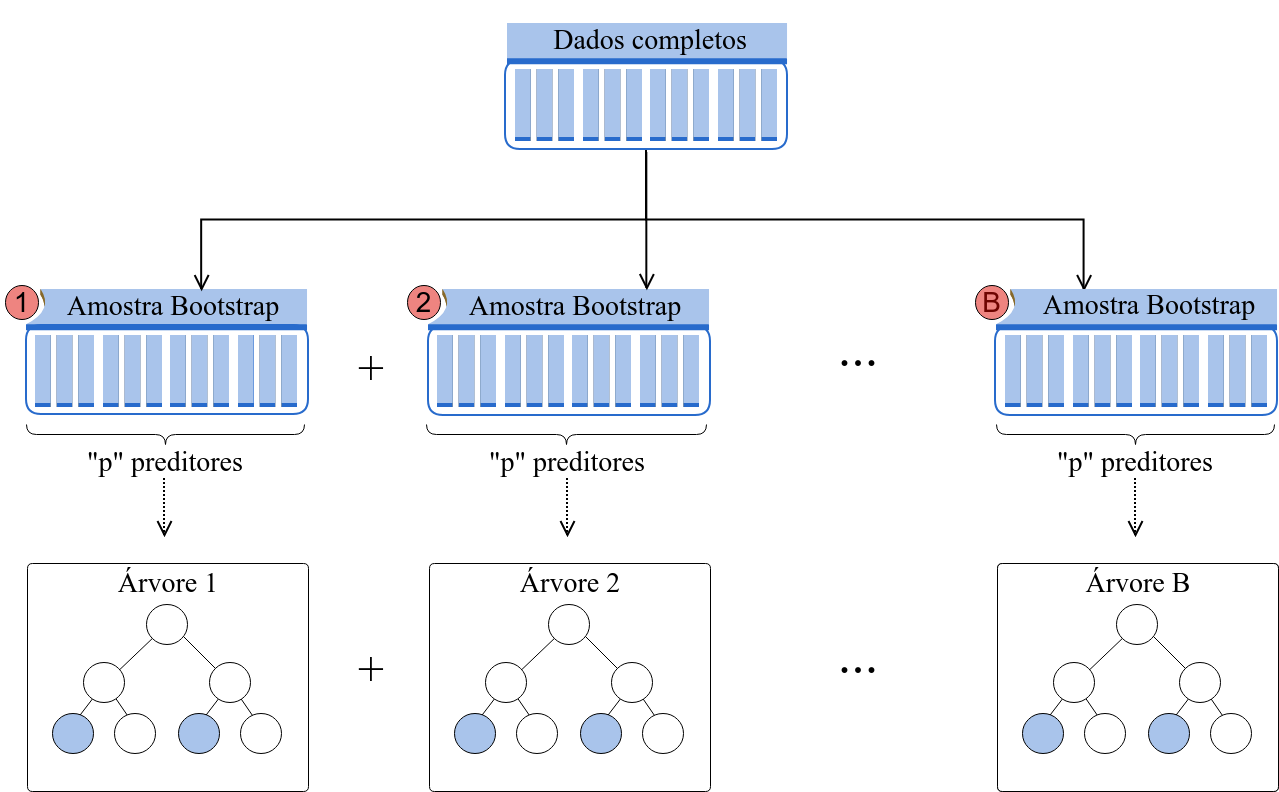
\includegraphics[keepaspectratio]{../../../images/regressao/bagging.png}}
\end{center}
\end{frame}

\begin{frame}
\begin{block}{Propriedade fundamental}
\phantomsection\label{propriedade-fundamental}
Se os estimadores são aproximadamente não viesados:

\begin{itemize}
\tightlist
\item
  o viés permanece semelhante\\
\item
  a variância é reduzida
\end{itemize}

Assim,

\[
\mathbb{E}[(\boldsymbol{y} - g(\mathbf{x}))^2 \mid \mathbf{x}]
\le
\mathbb{E}[(\boldsymbol{y} - g_b(\mathbf{x}))^2 \mid \mathbf{x}]
\]
\end{block}
\end{frame}

\begin{frame}
\begin{block}{Importância de Variáveis em Árvores}
\phantomsection\label{importuxe2ncia-de-variuxe1veis-em-uxe1rvores}
Bagging permite medir a relevância de cada variável:

\begin{itemize}
\tightlist
\item
  baseada na redução do erro (RSS)\\
\item
  cada divisão reduz a variabilidade
\end{itemize}

A qualidade de uma divisão é medida pela redução do erro quadrático
(RSS).

Considere um nó pai dividido em dois nós:

\begin{itemize}
\tightlist
\item
  esquerda (\(\mathcal{R}_{esq}\))\\
\item
  direita (\(\mathcal{R}_{dir}\))
\end{itemize}
\end{block}
\end{frame}

\begin{frame}
\begin{block}{Redução do erro}
\phantomsection\label{reduuxe7uxe3o-do-erro}
A redução no RSS é dada por:

\[
\text{RSS}_{pai}
-
\text{RSS}_{esq}
-
\text{RSS}_{dir}
\]

Ou, explicitamente:

\[
\sum_{i \in \mathcal{R}_{pai}} (y_i - \bar{y}_{pai})^2
-
\sum_{i \in \mathcal{R}_{esq}} (y_i - \bar{y}_{esq})^2
-
\sum_{i \in \mathcal{R}_{dir}} (y_i - \bar{y}_{dir})^2
\]
\end{block}
\end{frame}

\begin{frame}
\begin{block}{Interpretação}
\phantomsection\label{interpretauxe7uxe3o-5}
\begin{itemize}
\tightlist
\item
  quanto maior a redução → melhor a divisão\\
\item
  boas variáveis geram partições mais homogêneas
\end{itemize}

\begin{quote}
Variáveis importantes são aquelas que mais reduzem a variabilidade da
resposta.
\end{quote}
\end{block}
\end{frame}

\begin{frame}
\begin{center}
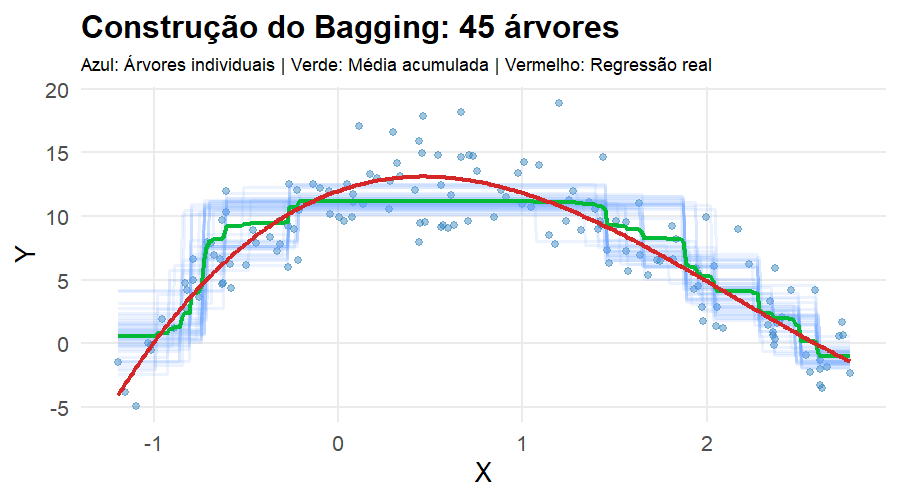
\includegraphics[width=0.9\linewidth,height=\textheight,keepaspectratio]{bagging_animado.png}
\end{center}
\end{frame}

\begin{frame}{Florestas Aleatórias (Random Forest)}
\phantomsection\label{florestas-aleatuxf3rias-random-forest}
No Bagging, combinamos várias árvores:

\[
g(\mathbf{x}) = \frac{1}{B} \sum_{b=1}^B g_b(\mathbf{x})
\]

Como as amostras \emph{bootstrap} não são \emph{i.i.d},

\begin{itemize}
\tightlist
\item
  Cada árvore é diferente, mas nasce do mesmo mecanismo, então têm
  variâncias semelhantes, ou seja,
\end{itemize}

\[
\mathrm{Var}(g_b(\mathbf{x})) = \sigma^2
\quad \text{para todo } b
\]
\end{frame}

\begin{frame}
\begin{itemize}
\tightlist
\item
  As árvores não são independentes, mas podemos resumir essa dependência
  por uma correlação média. Assim, a correlação entre quaisquer duas
  árvores é
\end{itemize}

\[
\mathrm{Cor}(g_b(\mathbf{x}),g_{b'}(\mathbf{x})) = \rho
\quad (b \neq b')
\]

Logo,

\[
\mathrm{Cov}(g_b(\mathbf{x}),g_{b'}(\mathbf{x})) = \rho \sigma^2
\]

Então,

\[
\mathrm{Var}\!\big(g(\mathbf{x}) \big)
=
\mathrm{Var}\!\left(\frac{1}{B}\sum_{b=1}^{B} g_b(\mathbf{x})\right)
=
\frac{1}{B^2}\mathrm{Var}\!\left(\sum_{b=1}^{B} g_b(\mathbf{x})\right)
\]
\end{frame}

\begin{frame}
Expandindo a variância da soma:

\[
\mathrm{Var}\!\left(\sum_{b=1}^{B} g_b(\mathbf{x})\right)
=
\sum_{b=1}^{B}\mathrm{Var}(g_b\big(\mathbf{x})\big)
+
\sum_{b \neq b'}\mathrm{Cov}\big(g_b(\mathbf{x}),g_{b'}(\mathbf{x})\big)
\]

Substituindo as hipóteses:

\[
\sum_{b=1}^{B}\mathrm{Var}\big(g_b(\mathbf{x})\big)=B\sigma^2
\]

e

\[
\sum_{b \neq b'}\mathrm{Cov}\big(g_b(\mathbf{x}),g_{b'}(\mathbf{x})\big)
=
B(B-1)\rho\sigma^2
\]
\end{frame}

\begin{frame}
Portanto,

\[
\mathrm{Var}\!\left(\sum_{b=1}^{B} g_b(\mathbf{x})\right)
=
B\sigma^2 + B(B-1)\rho\sigma^2
\]

e, assim,

\[
\mathrm{Var}\!\left(g(\mathbf{x})\right)
=
\frac{1}{B^2}
\left[
B\sigma^2 + B(B-1)\rho\sigma^2
\right]
\]
\end{frame}

\begin{frame}
Simplificando,

\[
\mathrm{Var}\!\big(g(\mathbf{x})\big)
=
\frac{\sigma^2}{B}
+
\frac{B-1}{B}\rho\sigma^2
\]

ou, equivalentemente,

\[
\boxed{
\mathrm{Var}\!\big(g(\mathbf{x})\big)
=
\rho\sigma^2 + \frac{1-\rho}{B}\sigma^2
}
\]

Note que,

\begin{itemize}
\tightlist
\item
  \(\rho\sigma^2\) é a parte da variância que \textbf{não desaparece}
  com o aumento de \(B\)
\item
  \(\dfrac{1-\rho}{B}\sigma^2\) é a parte que \textbf{cai com o número
  de árvores}
\end{itemize}
\end{frame}

\begin{frame}
\begin{block}{Consequência importante}
\phantomsection\label{consequuxeancia-importante}
\begin{itemize}
\tightlist
\item
  se \(\rho\) é pequeno, o bagging reduz bastante a variância
\item
  se \(\rho\) é grande, o ganho é limitado
\end{itemize}

Além disso,

\begin{itemize}
\tightlist
\item
  mesmas variáveis dominantes\\
\item
  divisões semelhantes\\
\item
  predições parecidas
\end{itemize}
\end{block}
\end{frame}

\begin{frame}
\begin{block}{Problema}
\phantomsection\label{problema}
A redução de variância depende da correlação:

\begin{quote}
árvores muito parecidas → pouco ganho ao combinar
\end{quote}
\end{block}

\begin{block}{Ideia do Random Forest}
\phantomsection\label{ideia-do-random-forest}
Introduzir aleatoriedade adicional:

\begin{quote}
em cada nó, escolhemos um subconjunto aleatório de variáveis
\end{quote}
\end{block}
\end{frame}

\begin{frame}
\begin{block}{Construção}
\phantomsection\label{construuxe7uxe3o}
Para cada árvore:

\begin{itemize}
\tightlist
\item
  amostra bootstrap dos dados
\item
  em cada divisão:

  \begin{itemize}
  \tightlist
  \item
    seleciona-se aleatoriamente \(m\) variáveis
  \item
    escolhe-se o melhor \emph{split} entre elas
  \end{itemize}
\end{itemize}
\end{block}

\begin{block}{Parâmetro chave}
\phantomsection\label{paruxe2metro-chave}
\begin{columns}[T]
\begin{column}{0.6\linewidth}
\(m\) = número de variáveis candidatas por \emph{split}

\begin{itemize}
\tightlist
\item
  \(m = d \rightarrow\) Bagging
\item
  \(m < d \rightarrow\) Random Forest
\end{itemize}
\end{column}

\begin{column}{0.4\linewidth}
\vspace{2.5cm}

\[
m \approx \frac{d}{3}
\]
\end{column}
\end{columns}
\end{block}
\end{frame}

\begin{frame}
\begin{center}
\pandocbounded{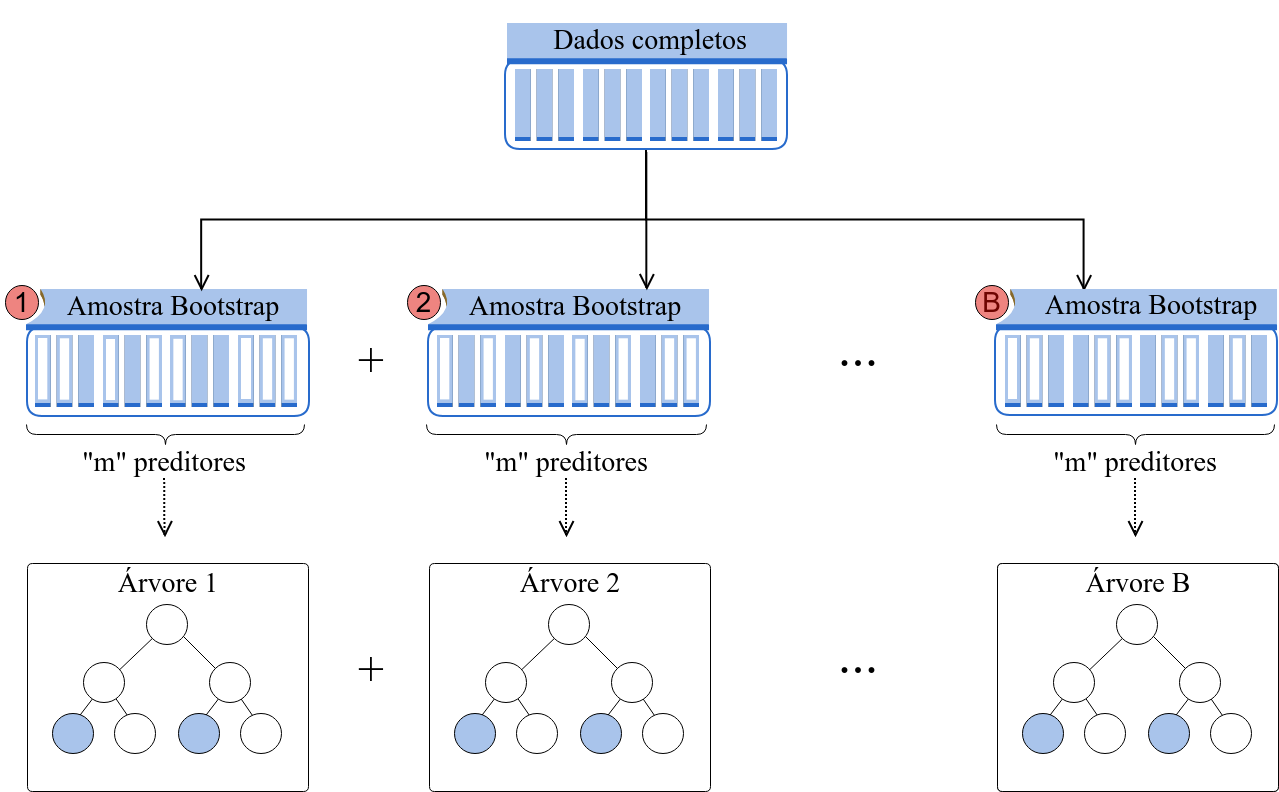
\includegraphics[keepaspectratio]{../../../images/regressao/rf.png}}
\end{center}
\end{frame}

\begin{frame}
\pandocbounded{
\includegraphics[keepaspectratio]{met_nao_param_files/figure-beamer/unnamed-chunk-10-1.png}}
\end{frame}

\begin{frame}
\begin{center}
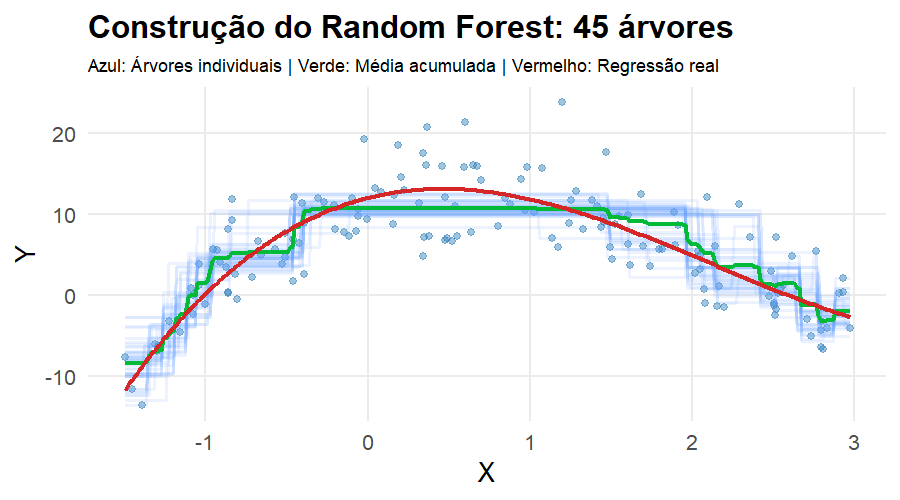
\includegraphics[width=0.9\linewidth,height=\textheight,keepaspectratio]{rf_animado.png}
\end{center}
\end{frame}

\begin{frame}{Boosting}
\phantomsection\label{boosting}
O \emph{boosting} constrói o estimador de forma \textbf{sequencial},
corrigindo erros do modelo anterior.

\begin{block}{Ideia central}
\phantomsection\label{ideia-central-2}
Começamos com um modelo simples e vamos \textbf{ajustando os resíduos}:

\[
r_i = y_i - g(x_i)
\]
\end{block}
\end{frame}

\begin{frame}
\begin{block}{Algoritmo}
\phantomsection\label{algoritmo}
\begin{enumerate}
\tightlist
\item
  Inicialize:
\end{enumerate}

\[
g(\mathbf{x}) = 0
\]

\begin{enumerate}
\setcounter{enumi}{1}
\tightlist
\item
  Para \(b = 1, \dots, B\):
\end{enumerate}

\begin{itemize}
\tightlist
\item
  Ajuste um modelo simples (ex: árvore rasa) aos resíduos:
\end{itemize}

\[
r_i = y_i - g(x_i)
\]

\begin{itemize}
\tightlist
\item
  Atualize:
\end{itemize}

\[
g(\mathbf{x}) \leftarrow g(\mathbf{x}) + \lambda g^{(b)}(\mathbf{x})
\]
\end{block}
\end{frame}

\begin{frame}
\begin{block}{Parâmetros importantes}
\phantomsection\label{paruxe2metros-importantes}
\begin{itemize}
\tightlist
\item
  \(B\) → número de iterações (\(B \approx 1000\))
\item
  \(\lambda\) → \emph{learning rate}, tipicamente pequeno
  (\(\lambda \approx 0,01\))

  \begin{itemize}
  \tightlist
  \item
    \(\lambda\) grande → aprendizado rápido → risco de overfitting
  \item
    \(\lambda\) pequeno → aprendizado lento → mais estável
  \end{itemize}
\item
  \(p\) → complexidade da árvore (\(p = 2\) ou \(p = 4\))
\end{itemize}
\end{block}

\begin{block}{Observação}
\phantomsection\label{observauxe7uxe3o}
\begin{itemize}
\tightlist
\item
  cada modelo aprende \textbf{o que o anterior errou}
\item
  reduz \textbf{viés} (diferente do bagging)
\end{itemize}
\end{block}
\end{frame}

\begin{frame}
\begin{center}
\pandocbounded{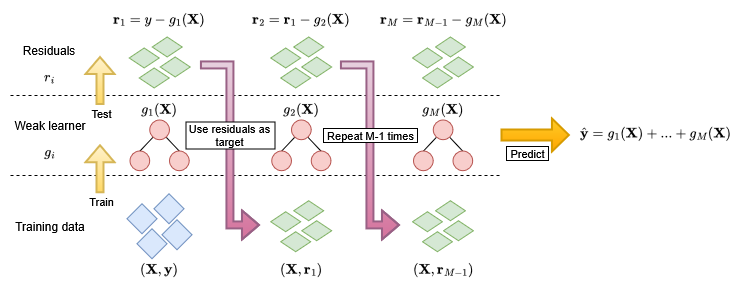
\includegraphics[keepaspectratio]{../../../images/regressao/boosting.png}}
\end{center}
\end{frame}

\begin{frame}
\pandocbounded{
\includegraphics[keepaspectratio]{met_nao_param_files/figure-beamer/unnamed-chunk-13-1.png}}
\end{frame}

\begin{frame}
\begin{center}
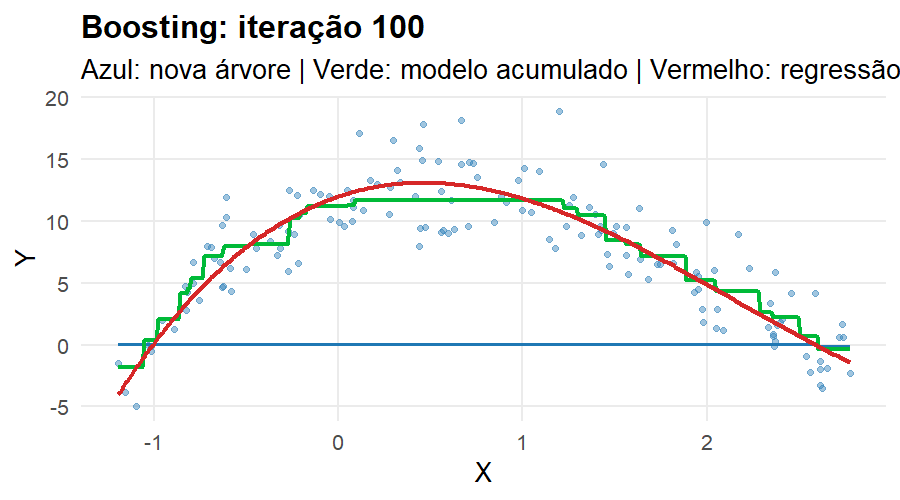
\includegraphics[width=0.9\linewidth,height=\textheight,keepaspectratio]{boosting_animado.png}
\end{center}
\end{frame}

\begin{frame}
\begin{block}{Boosting e Estimadores Fracos}
\phantomsection\label{boosting-e-estimadores-fracos}
O \emph{boosting} não é restrito ao uso de árvores.

Podemos usar qualquer modelo como base, desde que seja um
\textbf{estimador fraco}.

\begin{block}{O que é um estimador fraco?}
\phantomsection\label{o-que-uxe9-um-estimador-fraco}
\begin{itemize}
\tightlist
\item
  modelo simples
\item
  baixo poder preditivo individual
\item
  pequeno viés de ajuste
\end{itemize}

\textbf{Exemplos:} árvores rasas (\emph{stumps}), regressão linear
simples, modelos com poucos parâmetros
\end{block}
\end{block}
\end{frame}

\begin{frame}
\begin{block}{Por que usar modelos fracos?}
\phantomsection\label{por-que-usar-modelos-fracos}
\begin{itemize}
\tightlist
\item
  evitam overfitting em cada etapa
\item
  permitem correções graduais
\item
  tornam o aprendizado mais estável
\end{itemize}

Se você usar modelos muito complexos (ex: árvores profundas):

👉 boosting pode superajustar rapidamente
\end{block}
\end{frame}

\begin{frame}
\pandocbounded{
\includegraphics[keepaspectratio]{met_nao_param_files/figure-beamer/unnamed-chunk-16-1.png}}
\end{frame}

\begin{frame}{Redes Neurais Artificiais}
\phantomsection\label{redes-neurais-artificiais}
Redes neurais são modelos que aproximam funções não lineares complexas.

No contexto de regressão, trata-se de um estimador não linear de
\(r(\mathbf{x})\) que pode ser representado graficamente por uma
estrutura do tipo

\begin{center}
\pandocbounded{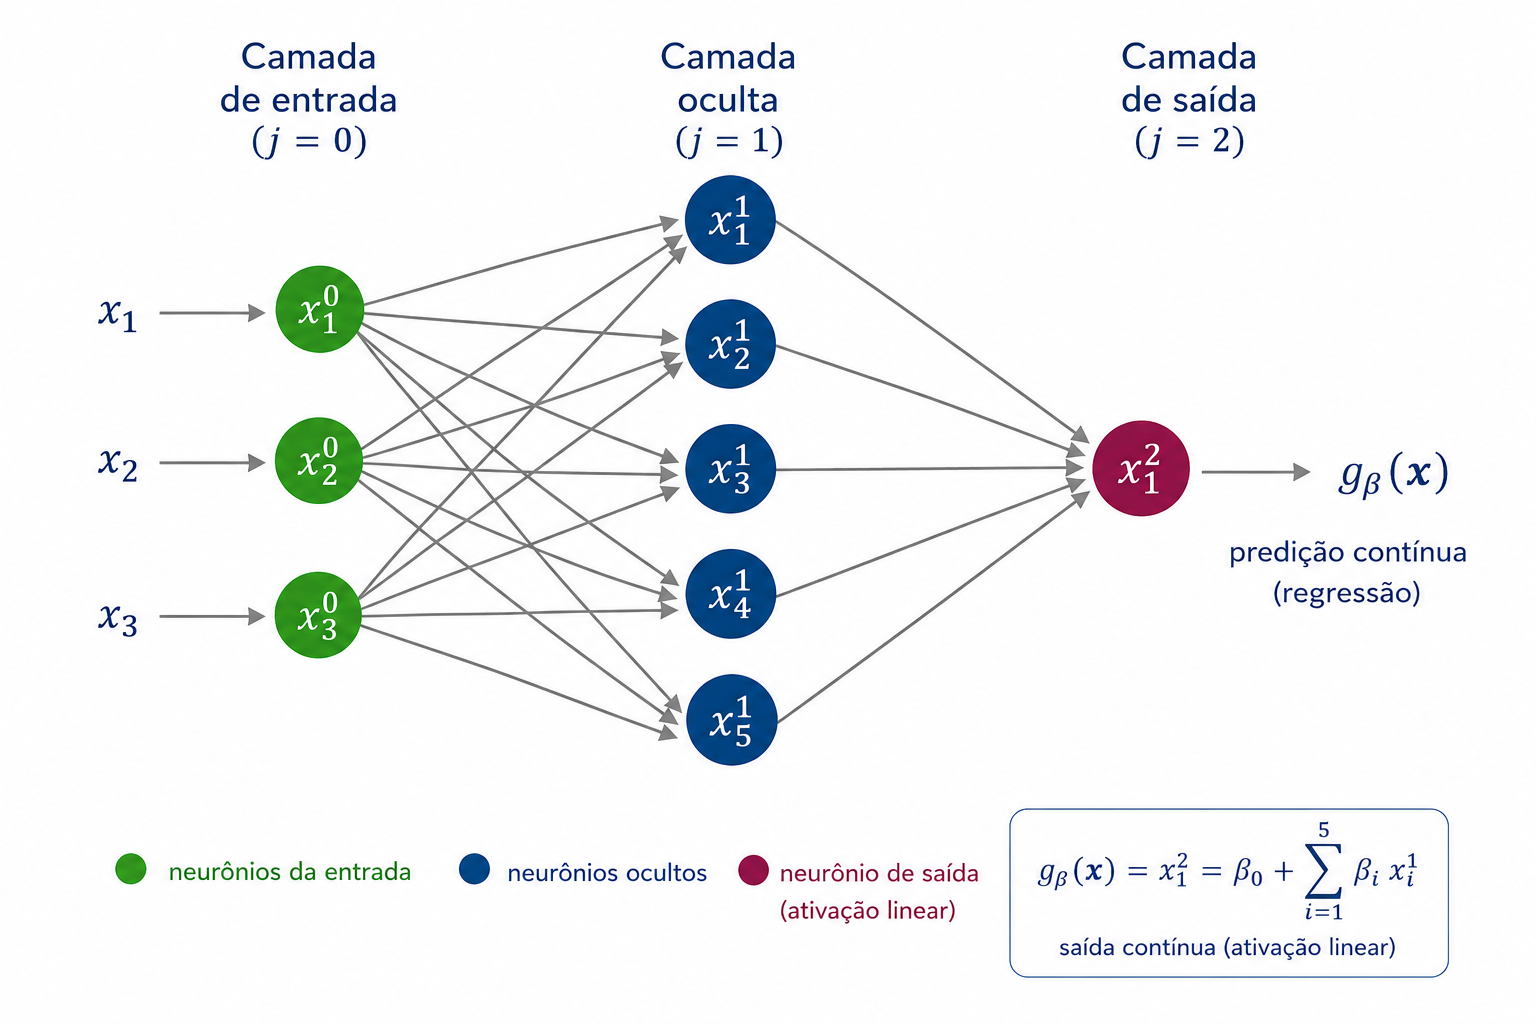
\includegraphics[keepaspectratio]{../../../images/regressao/rna.png}}
\end{center}
\end{frame}

\begin{frame}
\begin{block}{RNA sem camada oculta}
\phantomsection\label{rna-sem-camada-oculta}
\pandocbounded{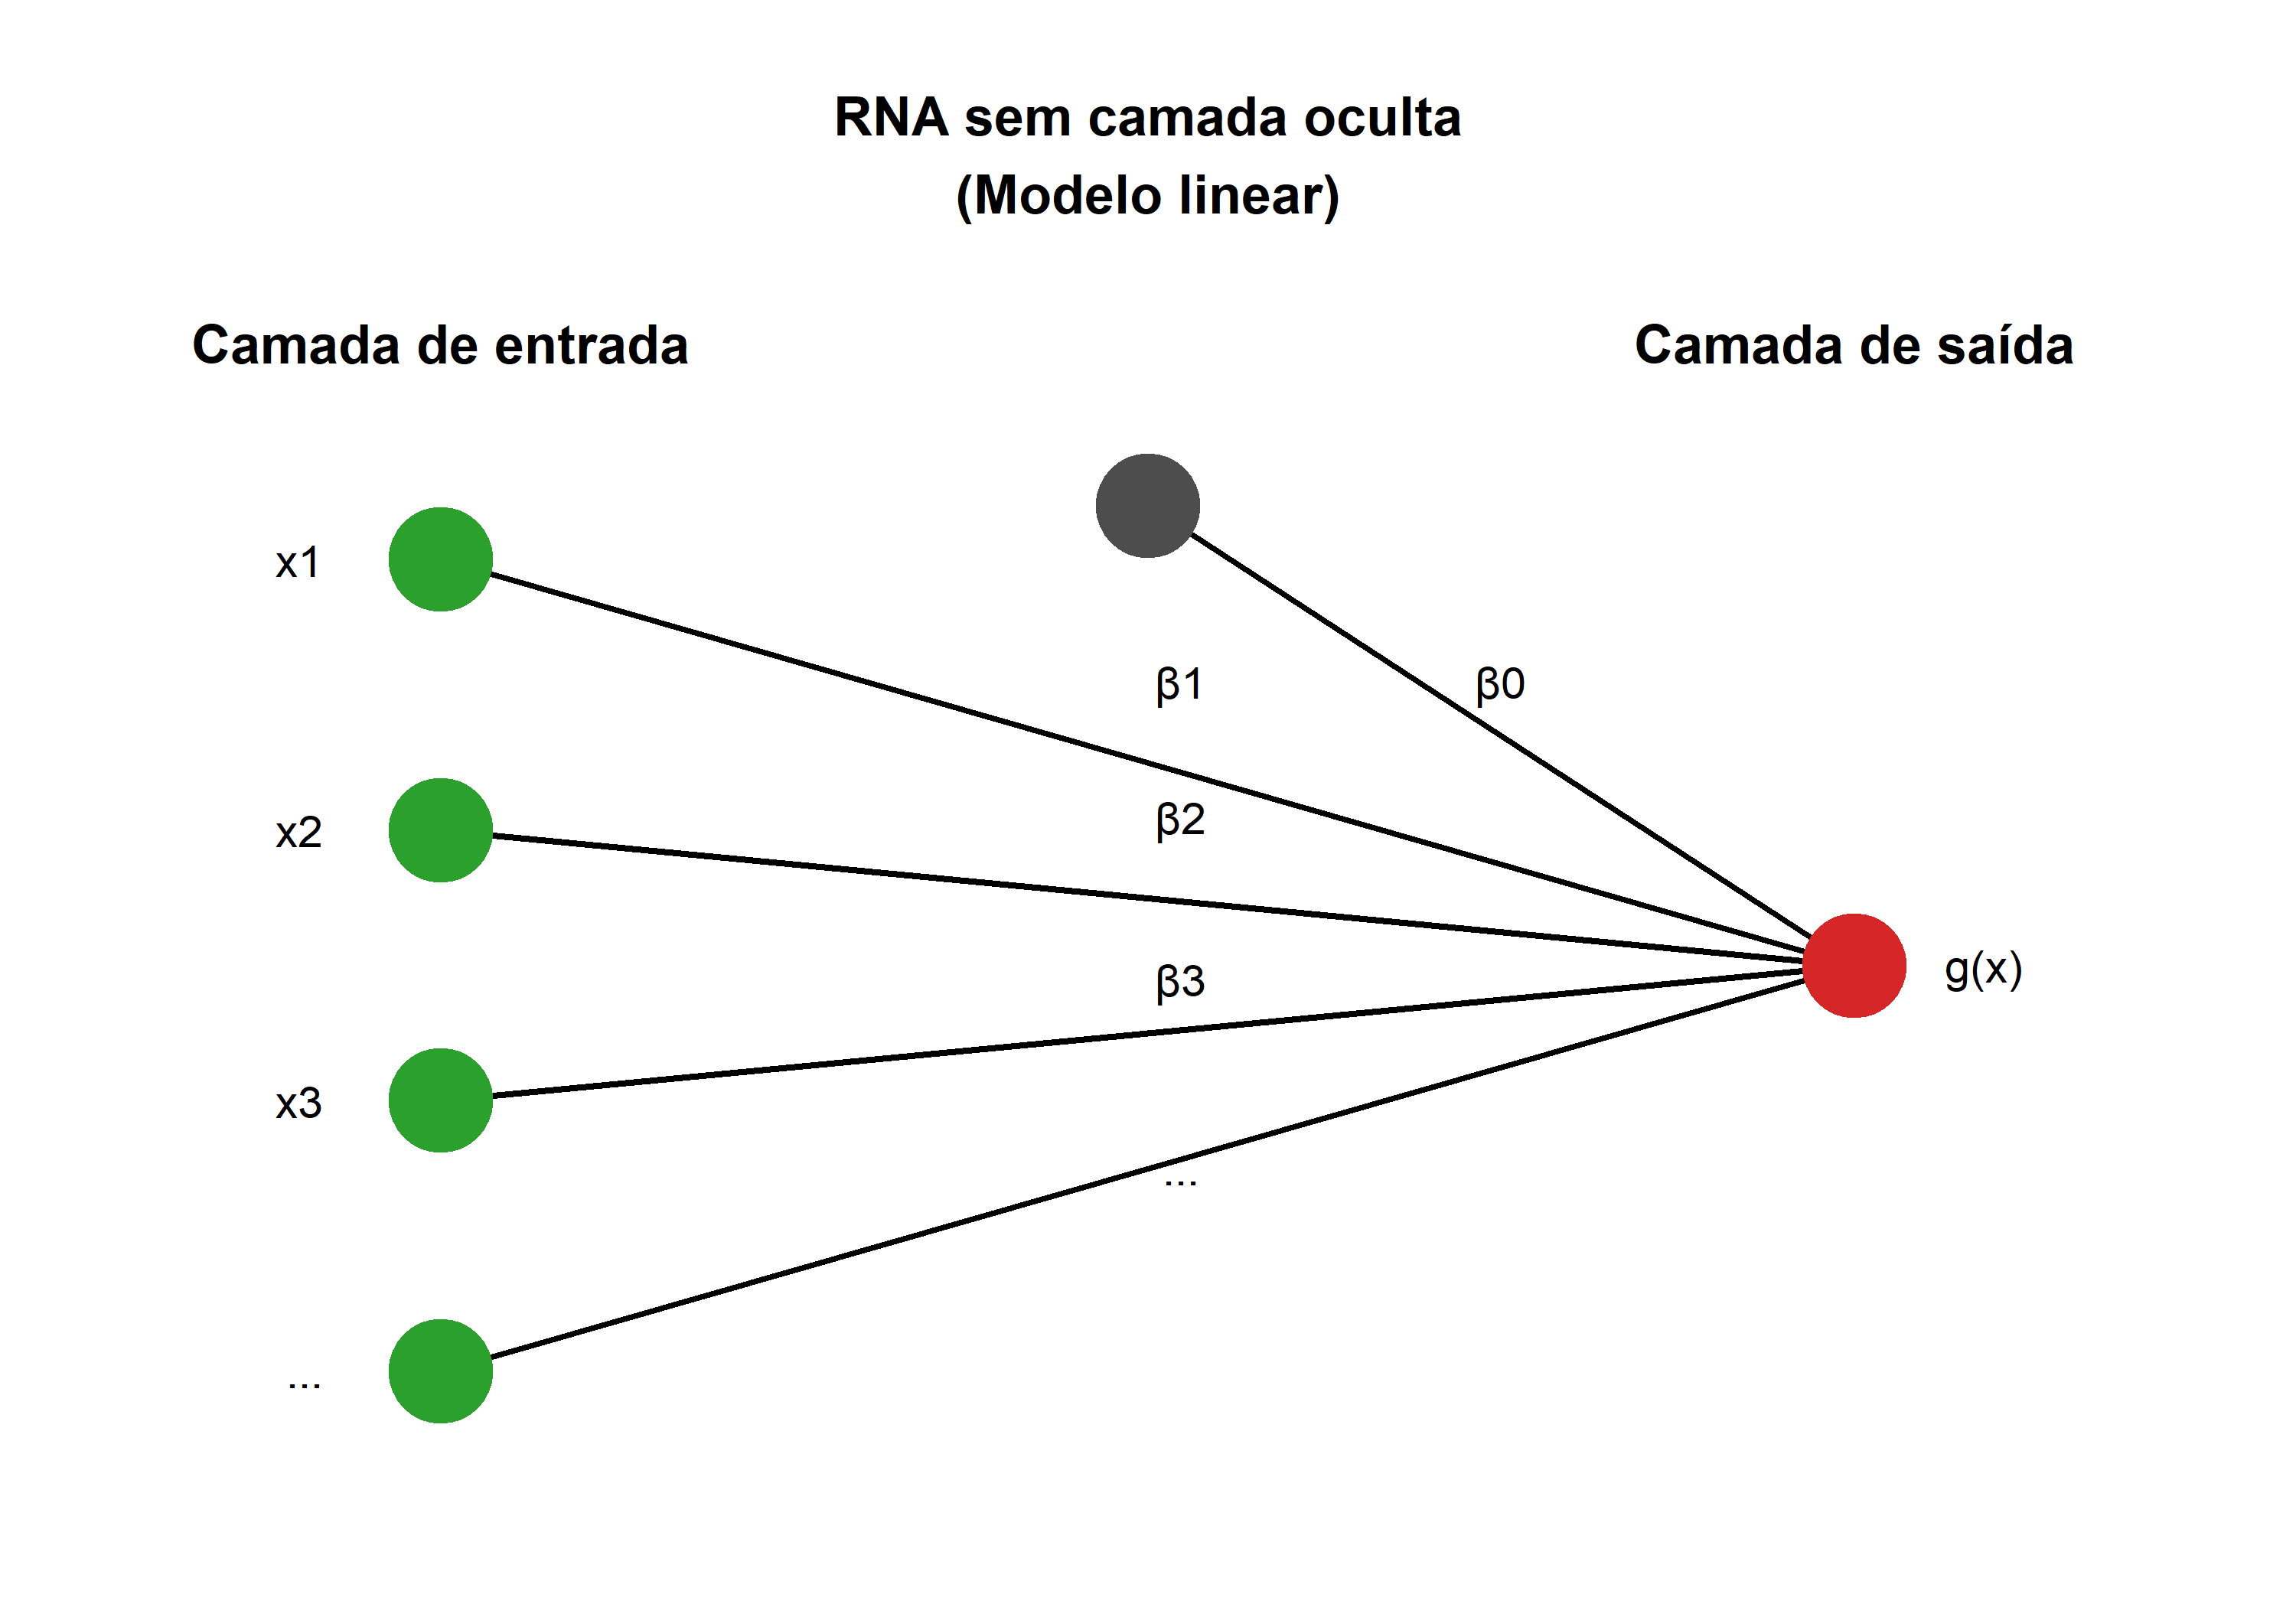
\includegraphics[keepaspectratio]{met_nao_param_files/figure-beamer/unnamed-chunk-17-1.png}}
\end{block}
\end{frame}

\begin{frame}
\begin{block}{🔹 Entrada}
\phantomsection\label{entrada}
\[
\mathbf{x} = (x_1, x_2, x_3, \cdots, x_p)^t
\]
\end{block}

\begin{block}{🔹 Camada de saída}
\phantomsection\label{camada-de-sauxedda}
\[
g(x) = f\left(\beta_0+\sum_{j=1}^{p} \beta_{j} x_j \right)
\]
\end{block}
\end{frame}

\begin{frame}
\begin{block}{RNA com camada oculta}
\phantomsection\label{rna-com-camada-oculta}
\begin{center}
\pandocbounded{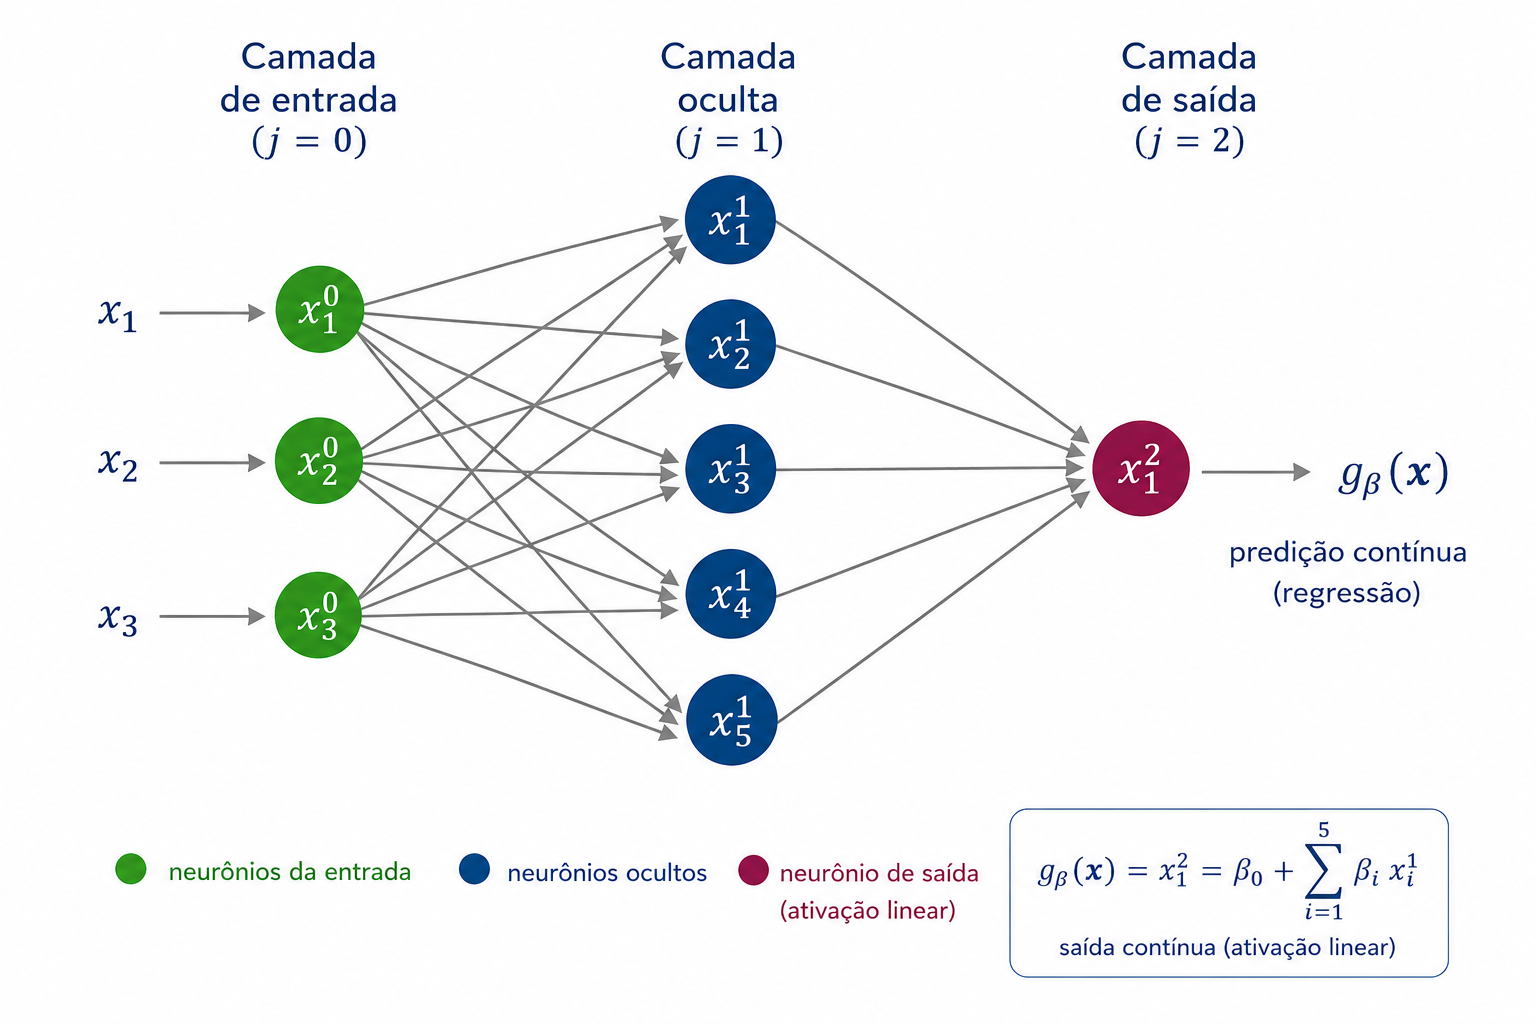
\includegraphics[keepaspectratio]{../../../images/regressao/rna.png}}
\end{center}
\end{block}
\end{frame}

\begin{frame}
Para a rede apresentada,

\begin{block}{🔹 Entrada}
\phantomsection\label{entrada-1}
\[
\mathbf{x} = (x_1, x_2, x_3)^t
\]
\end{block}

\begin{block}{🔹 Camada oculta}
\phantomsection\label{camada-oculta}
Um dado neurônio \(j\) da camada oculta é calculado como

\[
x_j^{1} = f\left( \beta_{0,j}^{(0)} + \sum_{i=1}^{3} \beta_{i,j}^{(0)} x_i^{0} \right),
\quad \text{com } x_i^{0} = x_i,\; i=1,2,3.
\]

e \(f\) é uma função definida pelo usuário, chamada de \textbf{função de
ativação.}
\end{block}
\end{frame}

\begin{frame}
\begin{block}{🔹 Saída}
\phantomsection\label{sauxedda}
\[
g(x) = x^{2}_1 = f\left( \beta_{0,1}^{1} + \sum_{i=1}^{5} \beta_{i,1}^{1} x_i^{1} \right)
\]
\end{block}
\end{frame}

\begin{frame}
\begin{block}{Representação de cada neurônio da rede}
\phantomsection\label{representauxe7uxe3o-de-cada-neuruxf4nio-da-rede}
\begin{center}
\pandocbounded{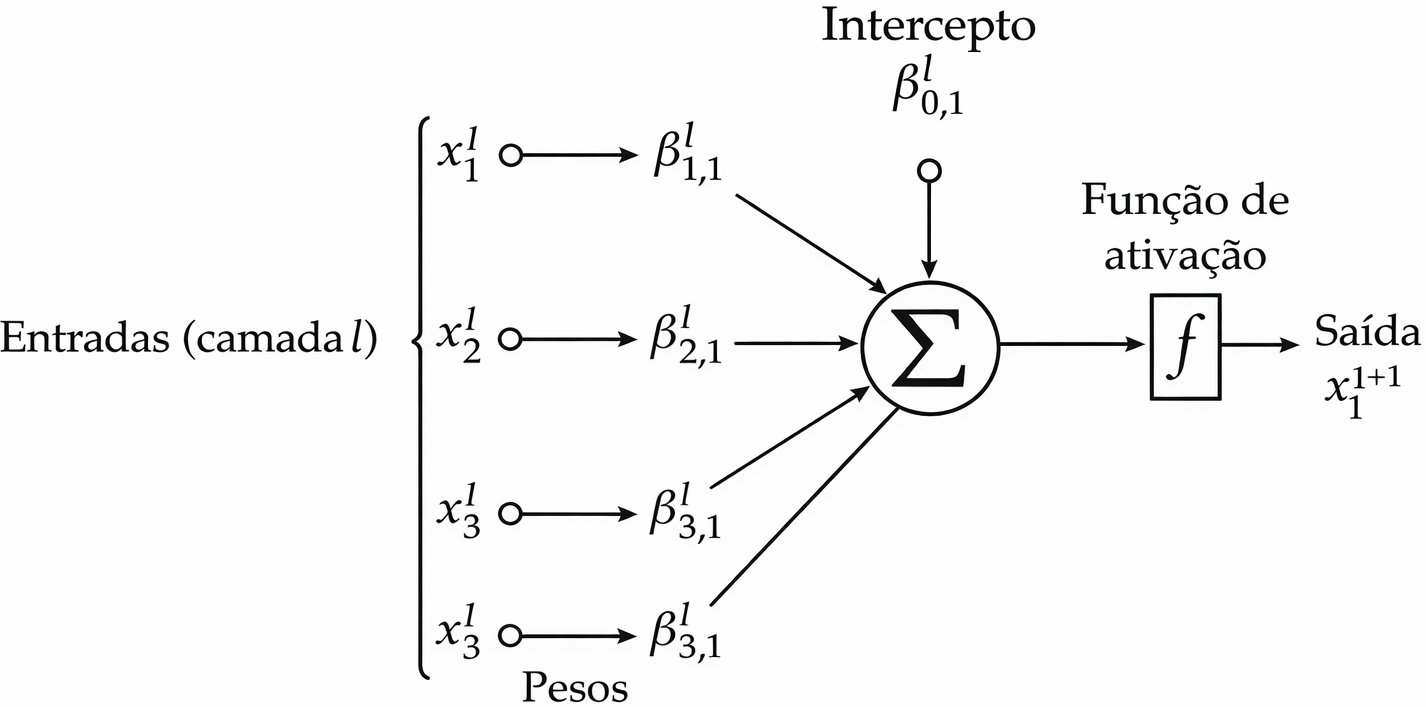
\includegraphics[keepaspectratio]{../../../images/regressao/neuronioMP2.png}}
\end{center}
\end{block}
\end{frame}

\begin{frame}
\begin{block}{Funções de Ativação}
\phantomsection\label{funuxe7uxf5es-de-ativauxe7uxe3o}
\begin{columns}[T]
\begin{column}{0.5\linewidth}
\begin{block}{Clássicas}
\phantomsection\label{cluxe1ssicas}
\begin{itemize}
\item
  Identidade \[
  f(z)=z
  \]
\item
  Sigmoid \[
  f(z)=\frac{1}{1+e^{-z}}
  \]
\item
  Tanh \[
  f(z)=\frac{e^z-e^{-z}}{e^z+e^{-z}}
  \]
\end{itemize}
\end{block}
\end{column}

\begin{column}{0.5\linewidth}
\begin{block}{Modernas}
\phantomsection\label{modernas}
\begin{itemize}
\item
  ReLU \[
  f(z)=\max(0,z)
  \]
\item
  Leaky ReLU \[
  f(z)=
  \begin{cases}
  0.01z, & z<0\\
  z, & z\geq0
  \end{cases}
  \]
\end{itemize}
\end{block}
\end{column}
\end{columns}
\end{block}
\end{frame}

\begin{frame}
\pandocbounded{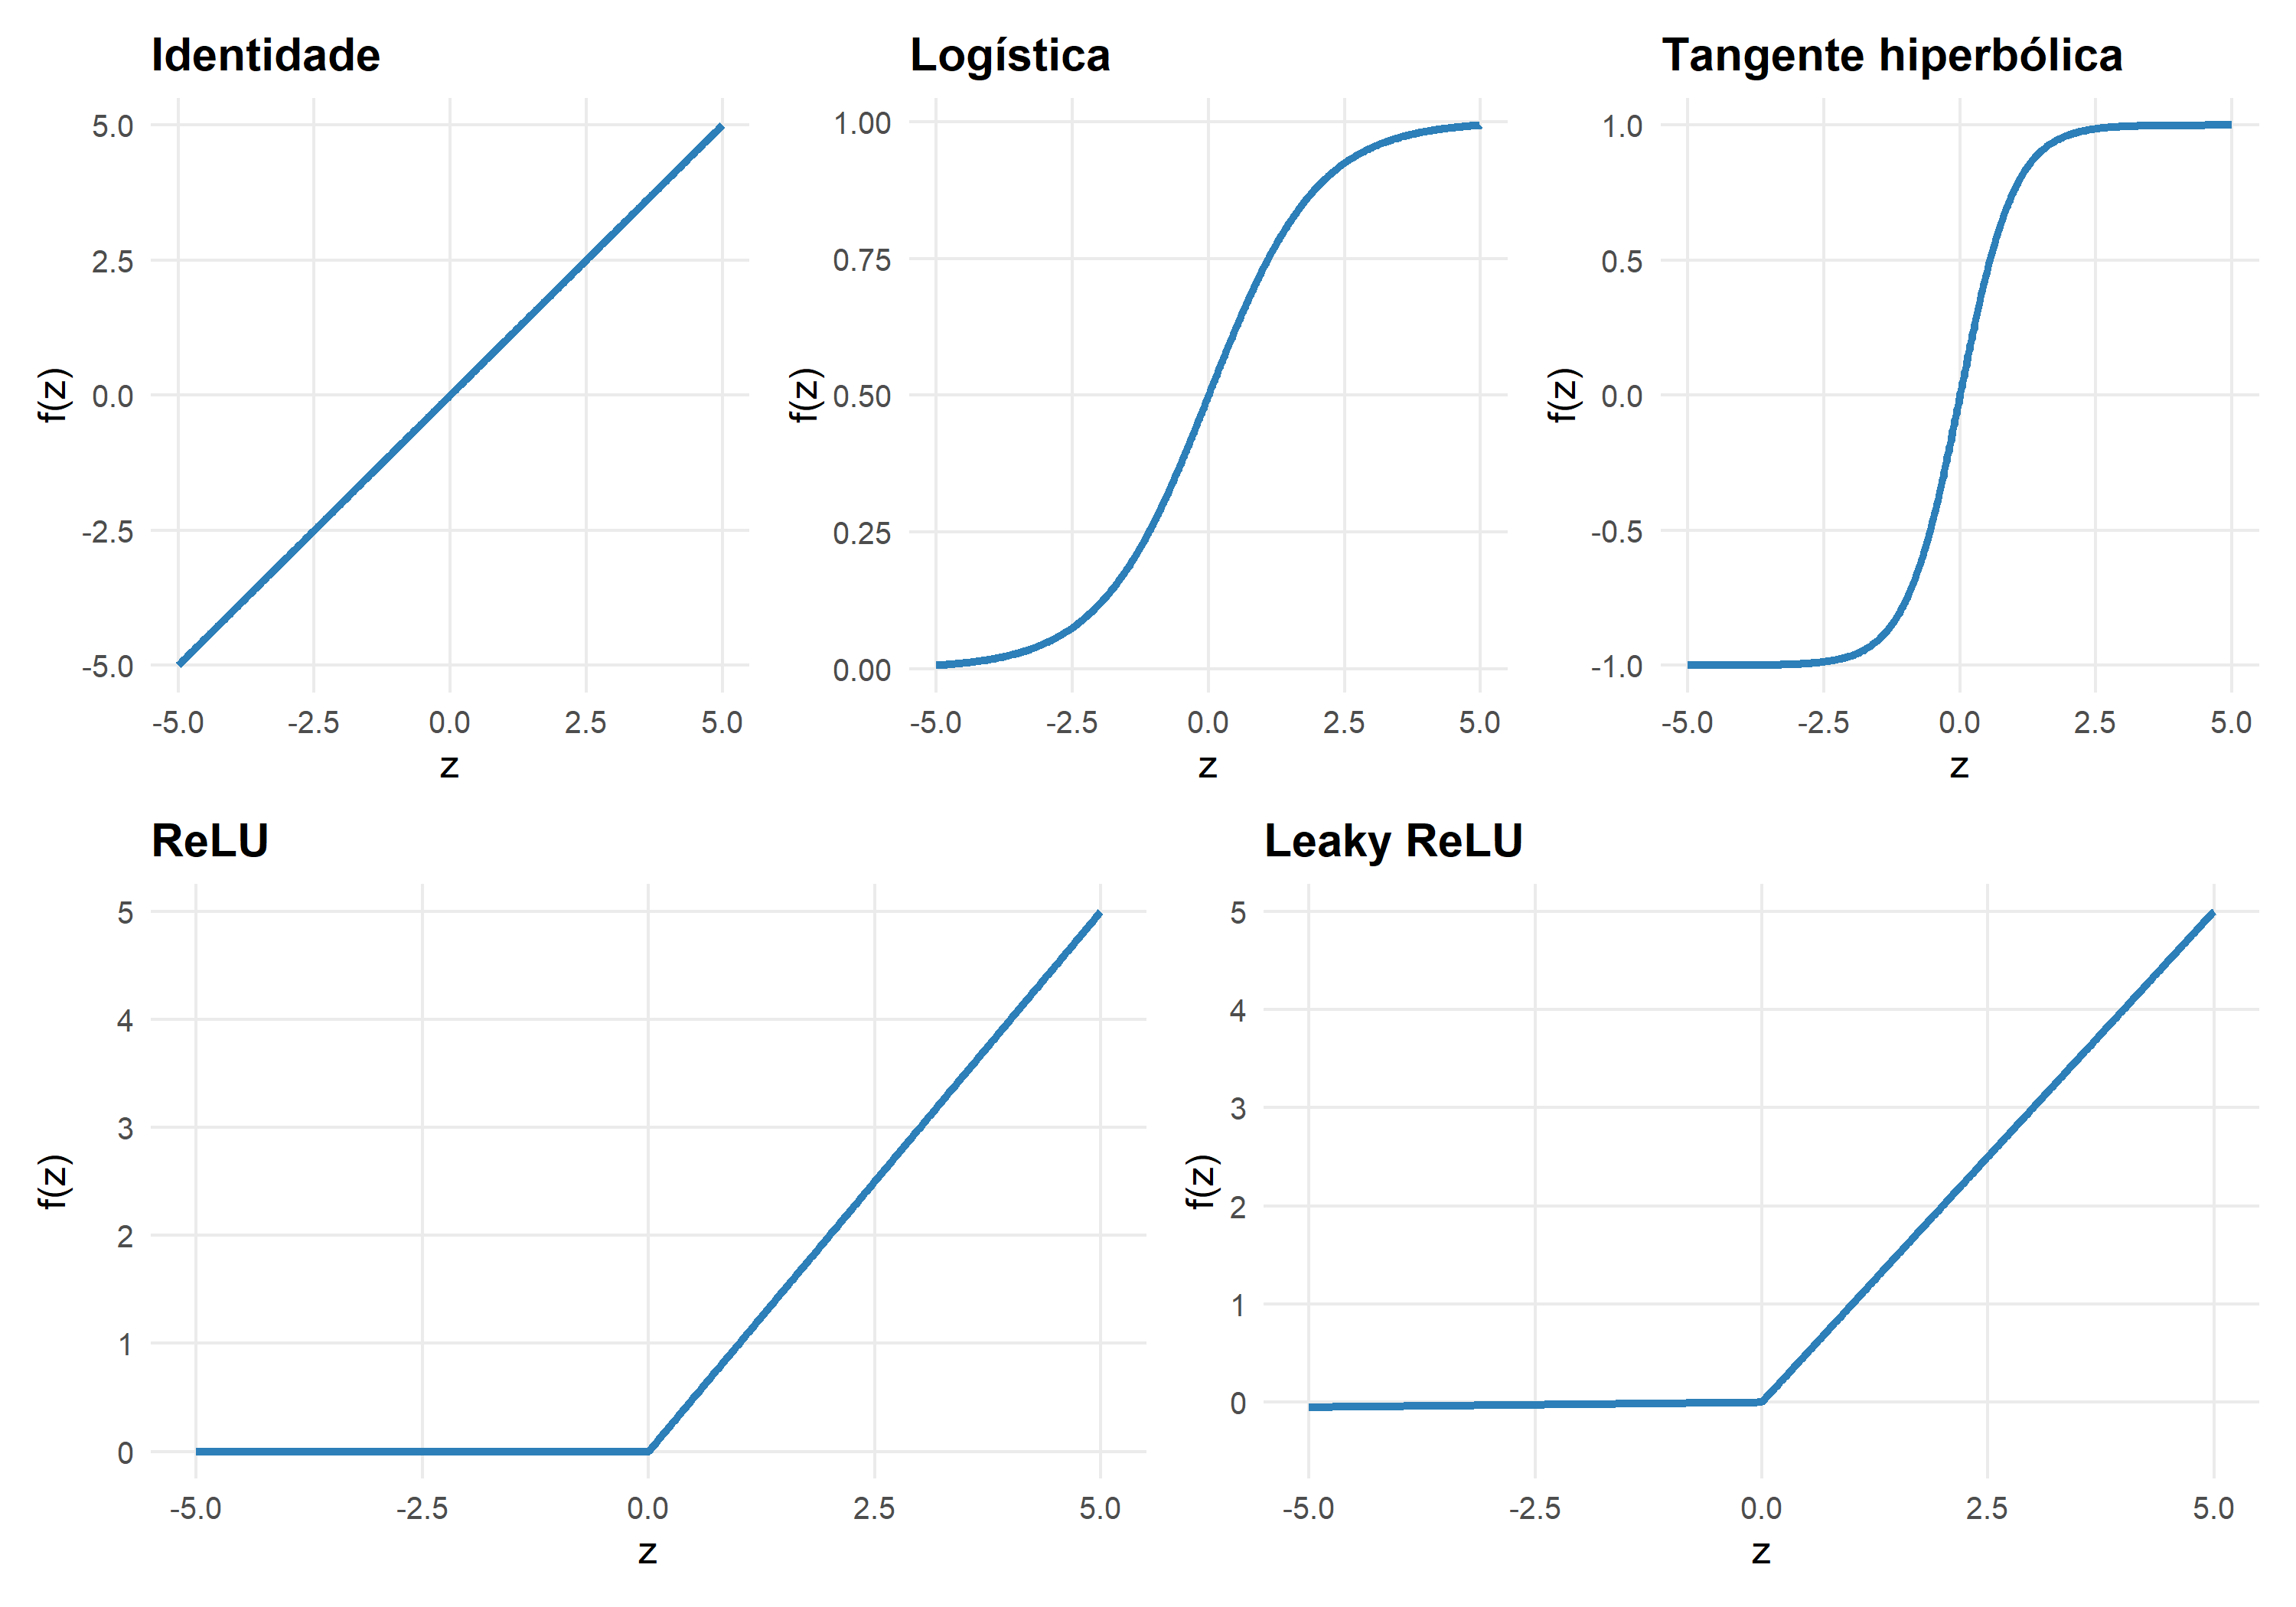
\includegraphics[keepaspectratio]{met_nao_param_files/figure-beamer/unnamed-chunk-18-1.png}}
\end{frame}

\begin{frame}
\pandocbounded{
\includegraphics[keepaspectratio]{met_nao_param_files/figure-beamer/unnamed-chunk-19-1.png}}
\end{frame}

\begin{frame}
\begin{block}{Por que precisamos de funções de ativação?}
\phantomsection\label{por-que-precisamos-de-funuxe7uxf5es-de-ativauxe7uxe3o}
Sem \(f(\cdot)\):

\[
g(\mathbf{x}) = \text{combinação linear}
\]

Com \(f(\cdot)\):

\[
g(\mathbf{x}) = \text{função não linear}
\]

A função de ativação é o que dá poder às redes neurais.
\end{block}
\end{frame}

\begin{frame}
\begin{block}{Estimação: Backpropagation}
\phantomsection\label{estimauxe7uxe3o-backpropagation}
Queremos estimar os parâmetros da rede neural, \(\beta\), minimizando o
erro:

\[
EQM(g_{\beta}) = \frac{1}{n} \sum_{k=1}^{n} (g_{\beta}(x_k) - y_k)^2
\]

\begin{block}{Problema}
\phantomsection\label{problema-1}
Não existe solução analítica.
\end{block}

\begin{block}{Solução}
\phantomsection\label{soluuxe7uxe3o}
Usamos \textbf{gradiente descendente}:

\[
\beta \leftarrow \beta - \eta \nabla EQM(g_\beta)
\]
\end{block}
\end{block}
\end{frame}

\begin{frame}
\begin{block}{Atualização dos pesos}
\phantomsection\label{atualizauxe7uxe3o-dos-pesos}
Para cada parâmetro:

\[
\beta_{i,j}^{(l)} \leftarrow 
\beta_{i,j}^{(l)} - \eta 
\frac{\partial EQM(g_\beta)}{\partial \beta_{i,j}^{(l)}}
\]

em que,

\begin{itemize}
\tightlist
\item
  \(\eta\) → taxa de aprendizado\\
\item
  \(l\) → camada\\
\item
  \((i,j)\) → conexão entre neurônios
\end{itemize}

Movemos os parâmetros na direção que \textbf{reduz o erro}
\end{block}
\end{frame}

\begin{frame}{Por que o nome Backpropagation?}
\phantomsection\label{por-que-o-nome-backpropagation}
Os gradientes são calculados da saída para a entrada

\begin{center}
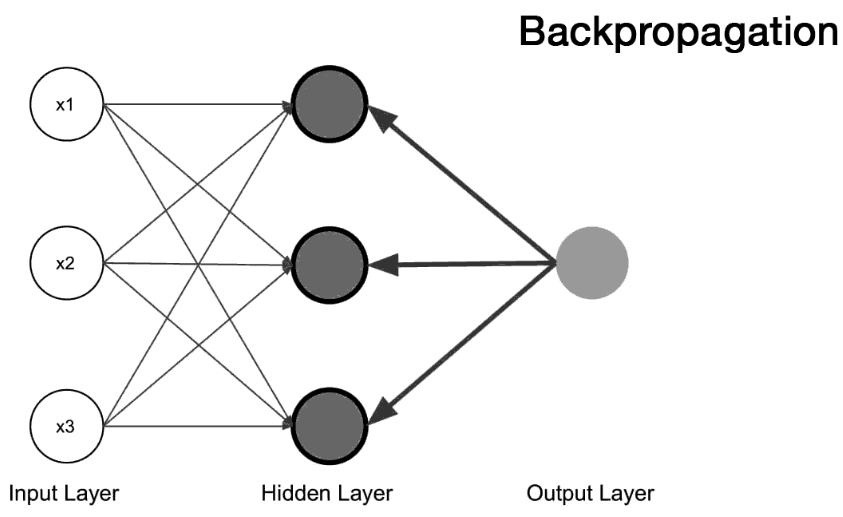
\includegraphics[width=0.6\linewidth,height=\textheight,keepaspectratio]{backpropagation.png}
\end{center}

O erro ``volta'' pela rede ajustando os pesos
\end{frame}

\begin{frame}
\begin{center}
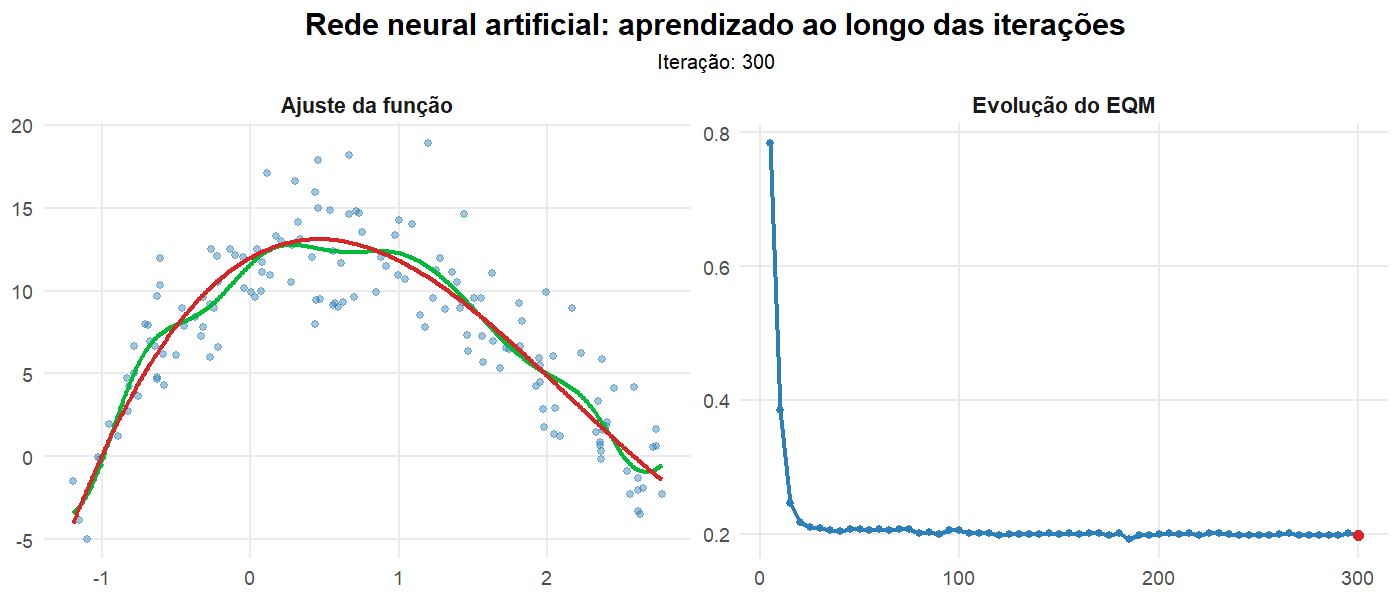
\includegraphics[width=1\linewidth,height=\textheight,keepaspectratio]{rna_eqm_lado_a_lado.png}
\end{center}
\end{frame}

\begin{frame}{Rede neural aprendendo uma função não linear}
\phantomsection\label{rede-neural-aprendendo-uma-funuxe7uxe3o-nuxe3o-linear}
Neste exemplo, a RNA foi ajustada para aproximar a função

\[
f(x)=12+4x-6x^2+x^3+\sin(x)
\]

a partir de observações ruidosas.

A curva verde mostra a predição da rede, enquanto a curva vermelha
representa a função real.
\end{frame}

\begin{frame}
\begin{block}{Síntese}
\phantomsection\label{suxedntese}
\begin{itemize}
\tightlist
\item
  a função de ativação introduz não linearidade;
\item
  a camada oculta cria novas representações dos dados;
\item
  o backpropagation ajusta os pesos para reduzir o erro;
\item
  com isso, a rede consegue aproximar funções complexas.
\end{itemize}
\end{block}
\end{frame}

\begin{frame}{References}
\phantomsection\label{references}
\phantomsection\label{refs}
\begin{CSLReferences}{1}{0}
\bibitem[\citeproctext]{ref-benedetti1977}
Benedetti, J. K. 1977. {``On the Nonparametric Estimation of Regression
Functions.''} \emph{Journal of the American Statistical Association}.

\bibitem[\citeproctext]{ref-stone1977}
Stone, Charles J. 1977. {``Consistent Nonparametric Regression.''}
\emph{The Annals of Statistics}.

\end{CSLReferences}
\end{frame}




\end{document}
